% Adapted from UH Manoa theme by:
% UH Manoa presentation theme for beamer
% Jeff Delmerico <jeffdelmerico@gmail.com> 2012
% https://github.com/jeffdelmerico/UH_Beamer_Theme.git


\documentclass{beamer}
%\documentclass[handout]{beamer}
\usetheme{PD}

\usepackage[absolute,overlay]{textpos}
\usepackage{helvet}
\usepackage{tikz}
\usepackage[italian]{babel}
\usepackage[utf8]{inputenc}

\usetikzlibrary{tikzmark,fit}

\title{Making Android run on time}
\subtitle{ }
\author{Matteo Di Pirro}
\date{26/07/2017}
\institute{Università degli Studi di Padova}

\begin{document}

\newcommand{\turnOffNumbers}{true} %hide frame numbers in footer

\begin{frame}[noframenumbering]
\titlepage
\end{frame}

\let\turnOffNumbers\empty
\begin{frame}
	\frametitle{Outline}
	\tableofcontents
\end{frame}

\section{Java e Android real-time}
\begin{frame}{Java e Android per real-time?}
	\begin{textblock*}{2cm}(7.5cm, 4cm)
		
\includegraphics[scale=0.1]{android}
	\end{textblock*}

	\begin{textblock*}{2cm}(1.5cm,2cm)
		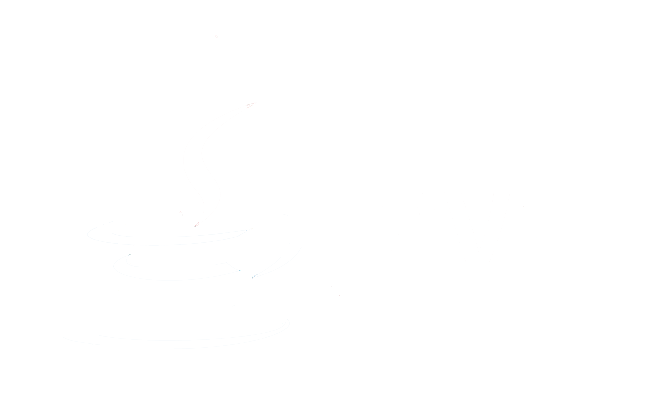
\includegraphics[scale=0.2]{java}
	\end{textblock*}
\end{frame}

\section{Java}
\subsection{Problematiche e soluzioni}
\begin{frame}{Limitazioni di Java real-time /1}
	\begin{itemize}
		\item Scheduling
		\begin{itemize}
			\item Nessun utilizzo delle priorità
			\begin{itemize}
				\item Nessuna garanzia che un thread ``critico'' venga eseguito
			\end{itemize}
		\end{itemize}
		\item Garbage collection
		\begin{itemize}
			\item Politica Stopping the world
			\begin{itemize}
				\item L'applicazione viene messa in pausa finché il GC pulisce la memoria
				\item Il ritardo introdotto è variabile e non quantificabile (dimensione della memoria, aggressività)
			\end{itemize}
			\item Tipicamente il ritardo varia da centinaia di ms a secondi, inaccettabile per applicazioni RT
		\end{itemize}
	\end{itemize}
\end{frame}
\begin{frame}{Limitazioni di Java real-time /2}
	\begin{itemize}
		\item Compilazione Just in time
		\begin{itemize}
			\item La VM compila in codice nativo i metodi eseguiti più frequentemente
			\begin{itemize}
				\item Start up veloce, ma non si sa quando verrà fatta la compilazione
				\item La compilazione è concorrente all'applicazione e provoca un ritardo non quantificabile
			\end{itemize}
			\item Viene migliorato il best case, ma la distanza tra BCET e WCET è molto elevata
			\begin{itemize}
				\item In un'applicazione RT quest'ultima dovrebbe essere il più piccola possibile per evitare WCET troppo pessimistici, che portano ad un utilizzo reale delle CPU troppo basso
			\end{itemize}
		\end{itemize}
	\end{itemize}
\end{frame}
\begin{frame}{Real-Time specification for Java \\e altre soluzioni}
	\begin{itemize}
		\item Scheduling
		\begin{itemize}
			\item Utilizzo reale delle priorità
			\item Basic Priority Inheritance Protocol
			\item Ceiling Priority Protocol (opzionale)
		\end{itemize}
		\item Gestione della memoria
		\begin{itemize}
			\item Scoped
			\item Immortal
		\end{itemize}
		\item Compilazione Ahead of time
		\begin{itemize}
			\item Maggiore prevedibilità
		\end{itemize}
	\end{itemize}
\end{frame}

\section{Android}
\subsection{Problematiche}
\begin{frame}{Limitazioni di Android real-time /1}
	\begin{itemize}
		\item La memoria disponibile è generalmente poca
		\begin{itemize}
			\item Garbage collection molto aggressiva
			\item La politica resta stopping the world, e la maggiore aggressività implica che i ritardi introdotti sono maggiori
			\item Se la memoria disponibile è molto bassa, la ``coda'' dei pronti viene salvata in memoria secondaria
			\begin{itemize}
				\item Il tempo richiesto per lo scheduling diventa così altissimo
			\end{itemize}
		\end{itemize}
	\end{itemize}
\end{frame}
\begin{frame}{Limitazioni di Android real-time /2}
	\begin{itemize}
		\item Completely Fair Scheduler
		\begin{itemize}
			\item La coda dei pronti è gestita con un albero rosso nero
			\begin{itemize}
				\item Costo $O(log(n))$ per inserimenti e cancellazioni, molto maggiore di $O(1)$ richiesto da un array indicizzato per priorità
				\item Costo maggiore per la memorizzazione in memoria
			\end{itemize}
			\item CFS ha come obiettivo la fairness, in contrasto con i sistemi real-time
			\begin{itemize}
				\item Un thread ad alta priorità può essere ``scavalcato'' da uno a priorità molto più bassa
				\item Non si tiene conto delle deadlines
			\end{itemize}
			\item Due politiche real-time sono supportate dal kernel Linux di Android
			\begin{itemize}
				\item \texttt{SCHED\_FIFO}
				\item \texttt{SCHED\_RR}
			\end{itemize}
			ma di default viene utilizzata \texttt{SCHED\_OTHER}, che non tiene conto della priorità
		\end{itemize}
	\end{itemize}
\end{frame}
\begin{frame}{Limitazioni di Android real-time /3}
	\only<1>{
		\begin{textblock*}{10cm}(2.7cm, 3.5cm)
			struct sched\_entity \{ \\
			\mbox{~~~~}... \\
			\mbox{~~~~}u64 exec\_start;\\
			\mbox{~~~~}u64 sum\_exec\_runtime;\\
			\mbox{~~~~}u64 vruntime;\\
			\mbox{~~~~}u64 prev\_sum\_exec\_runtime;\\
			\mbox{~~~~}...\\
			\}
		\end{textblock*}
	}
	\only<2>{
		\begin{textblock*}{10cm}(2.7cm, 3cm)
			struct sched\_entity \{\\
			\mbox{~~~~}... \\
			\mbox{~~~~}u64 exec\_start;\\
			\mbox{~~~~}u64 sum\_exec\_runtime;\\
			\mbox{~~~~}u64 vruntime;\\
			\mbox{~~~~}u64 prev\_sum\_exec\_runtime;\\
			\mbox{~~~~}...\\
			\}
		\end{textblock*}
		\begin{textblock*}{10cm}(2.7cm, 7cm)
			$delta\_exec\_weighted = delta\_exec * \frac{NICE\_0\_LOAD}{load\_weight}$
		\end{textblock*}
	}
\end{frame}
\begin{frame}{Limitazioni di Android real-time /4}
	\begin{itemize}
		\item Scambio di messaggi
		\begin{itemize}
			\item \texttt{Handler} e \texttt{Looper}
			\begin{itemize}
				\item Nessun supporto delle priorità
				\item Coda ordinata dinamicamente: un messaggio proveniente da un thread ad alta priorità non ha garanzia di essere ricevuto velocemente
			\end{itemize}
		\end{itemize}
		\item Servizi di sistema
		\begin{itemize}
			\item \texttt{AlarmManager}
			\begin{itemize}
				\item Nessuna garanzia sul tempo di notifica
			\end{itemize}
			\item \texttt{SensorManager}
			\begin{itemize}
				\item Nessun supporto alle priorità: thread a priorità più alta possono essere notificati dopo thread a priorità bassa
				\item La notifica utilizza \texttt{Handler} e \texttt{Looper}, con ritardi variabili
			\end{itemize}
		\end{itemize}
	\end{itemize}
\end{frame}
\begin{frame}{Handler e Looper}
	\vspace{-10px}
	\centering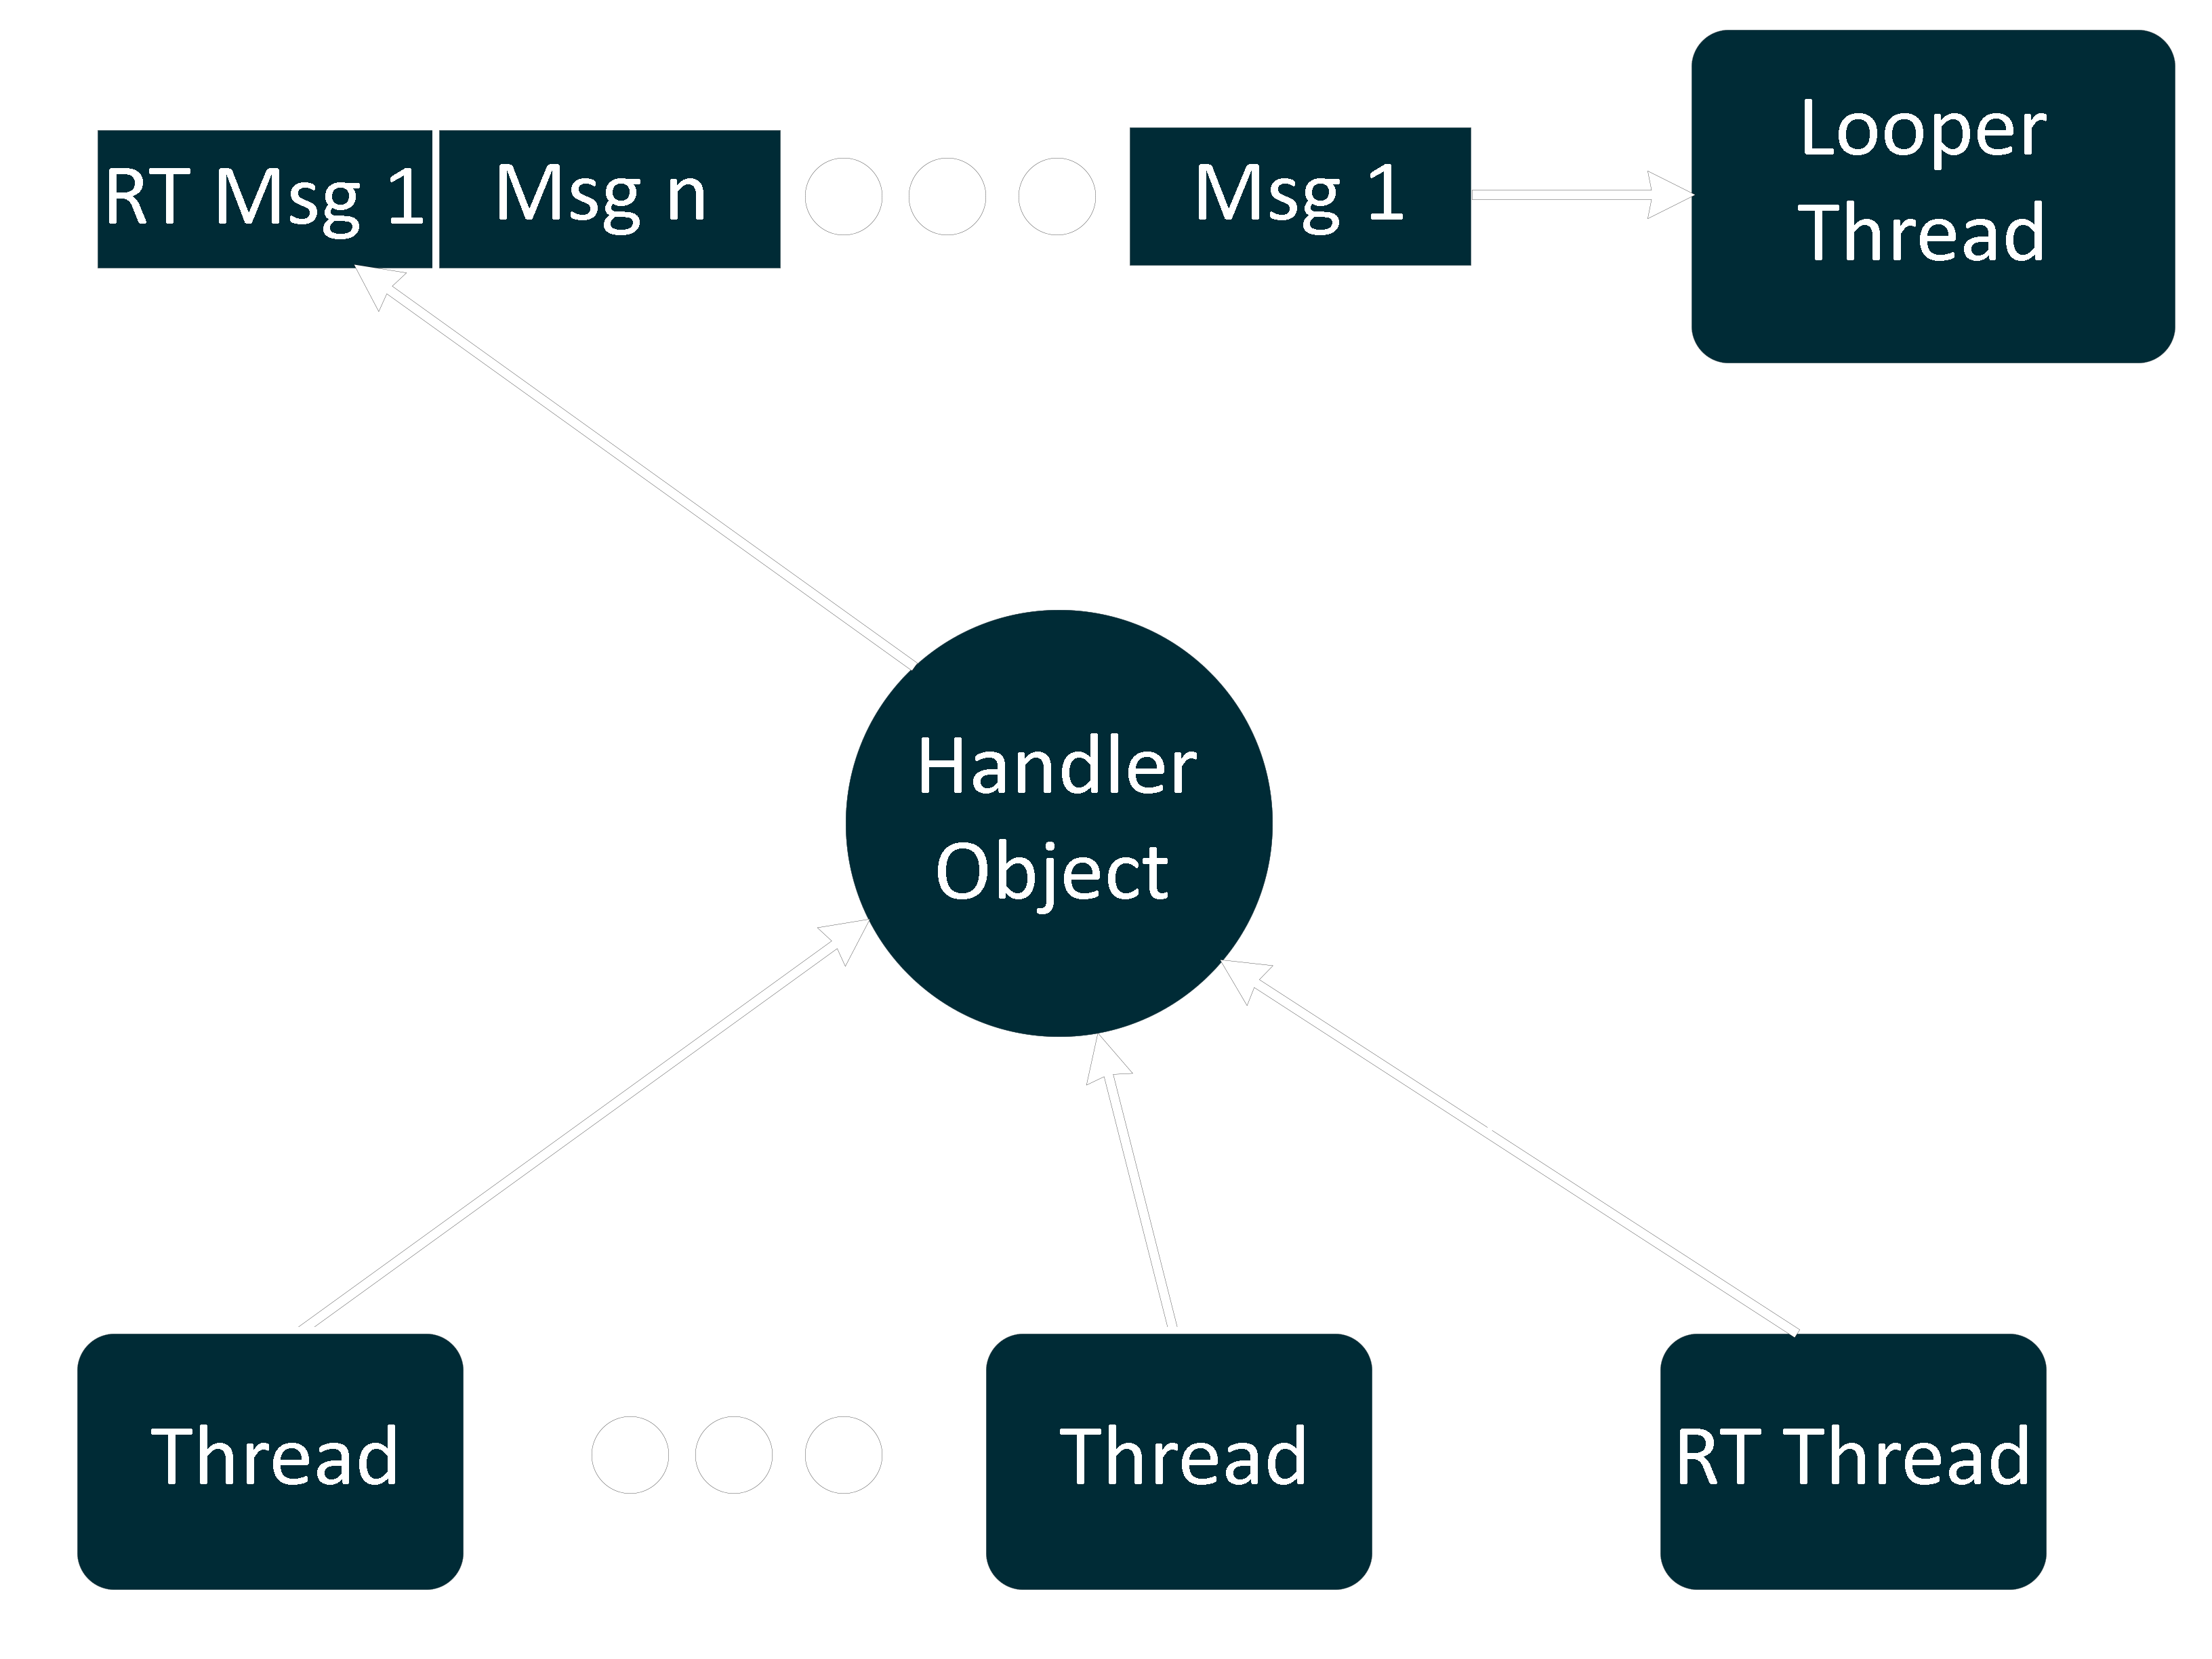
\includegraphics[scale=0.08]{handlerLooper}
\end{frame}
\begin{frame}{Fonti di jitter}
 	\vspace{-10px}
	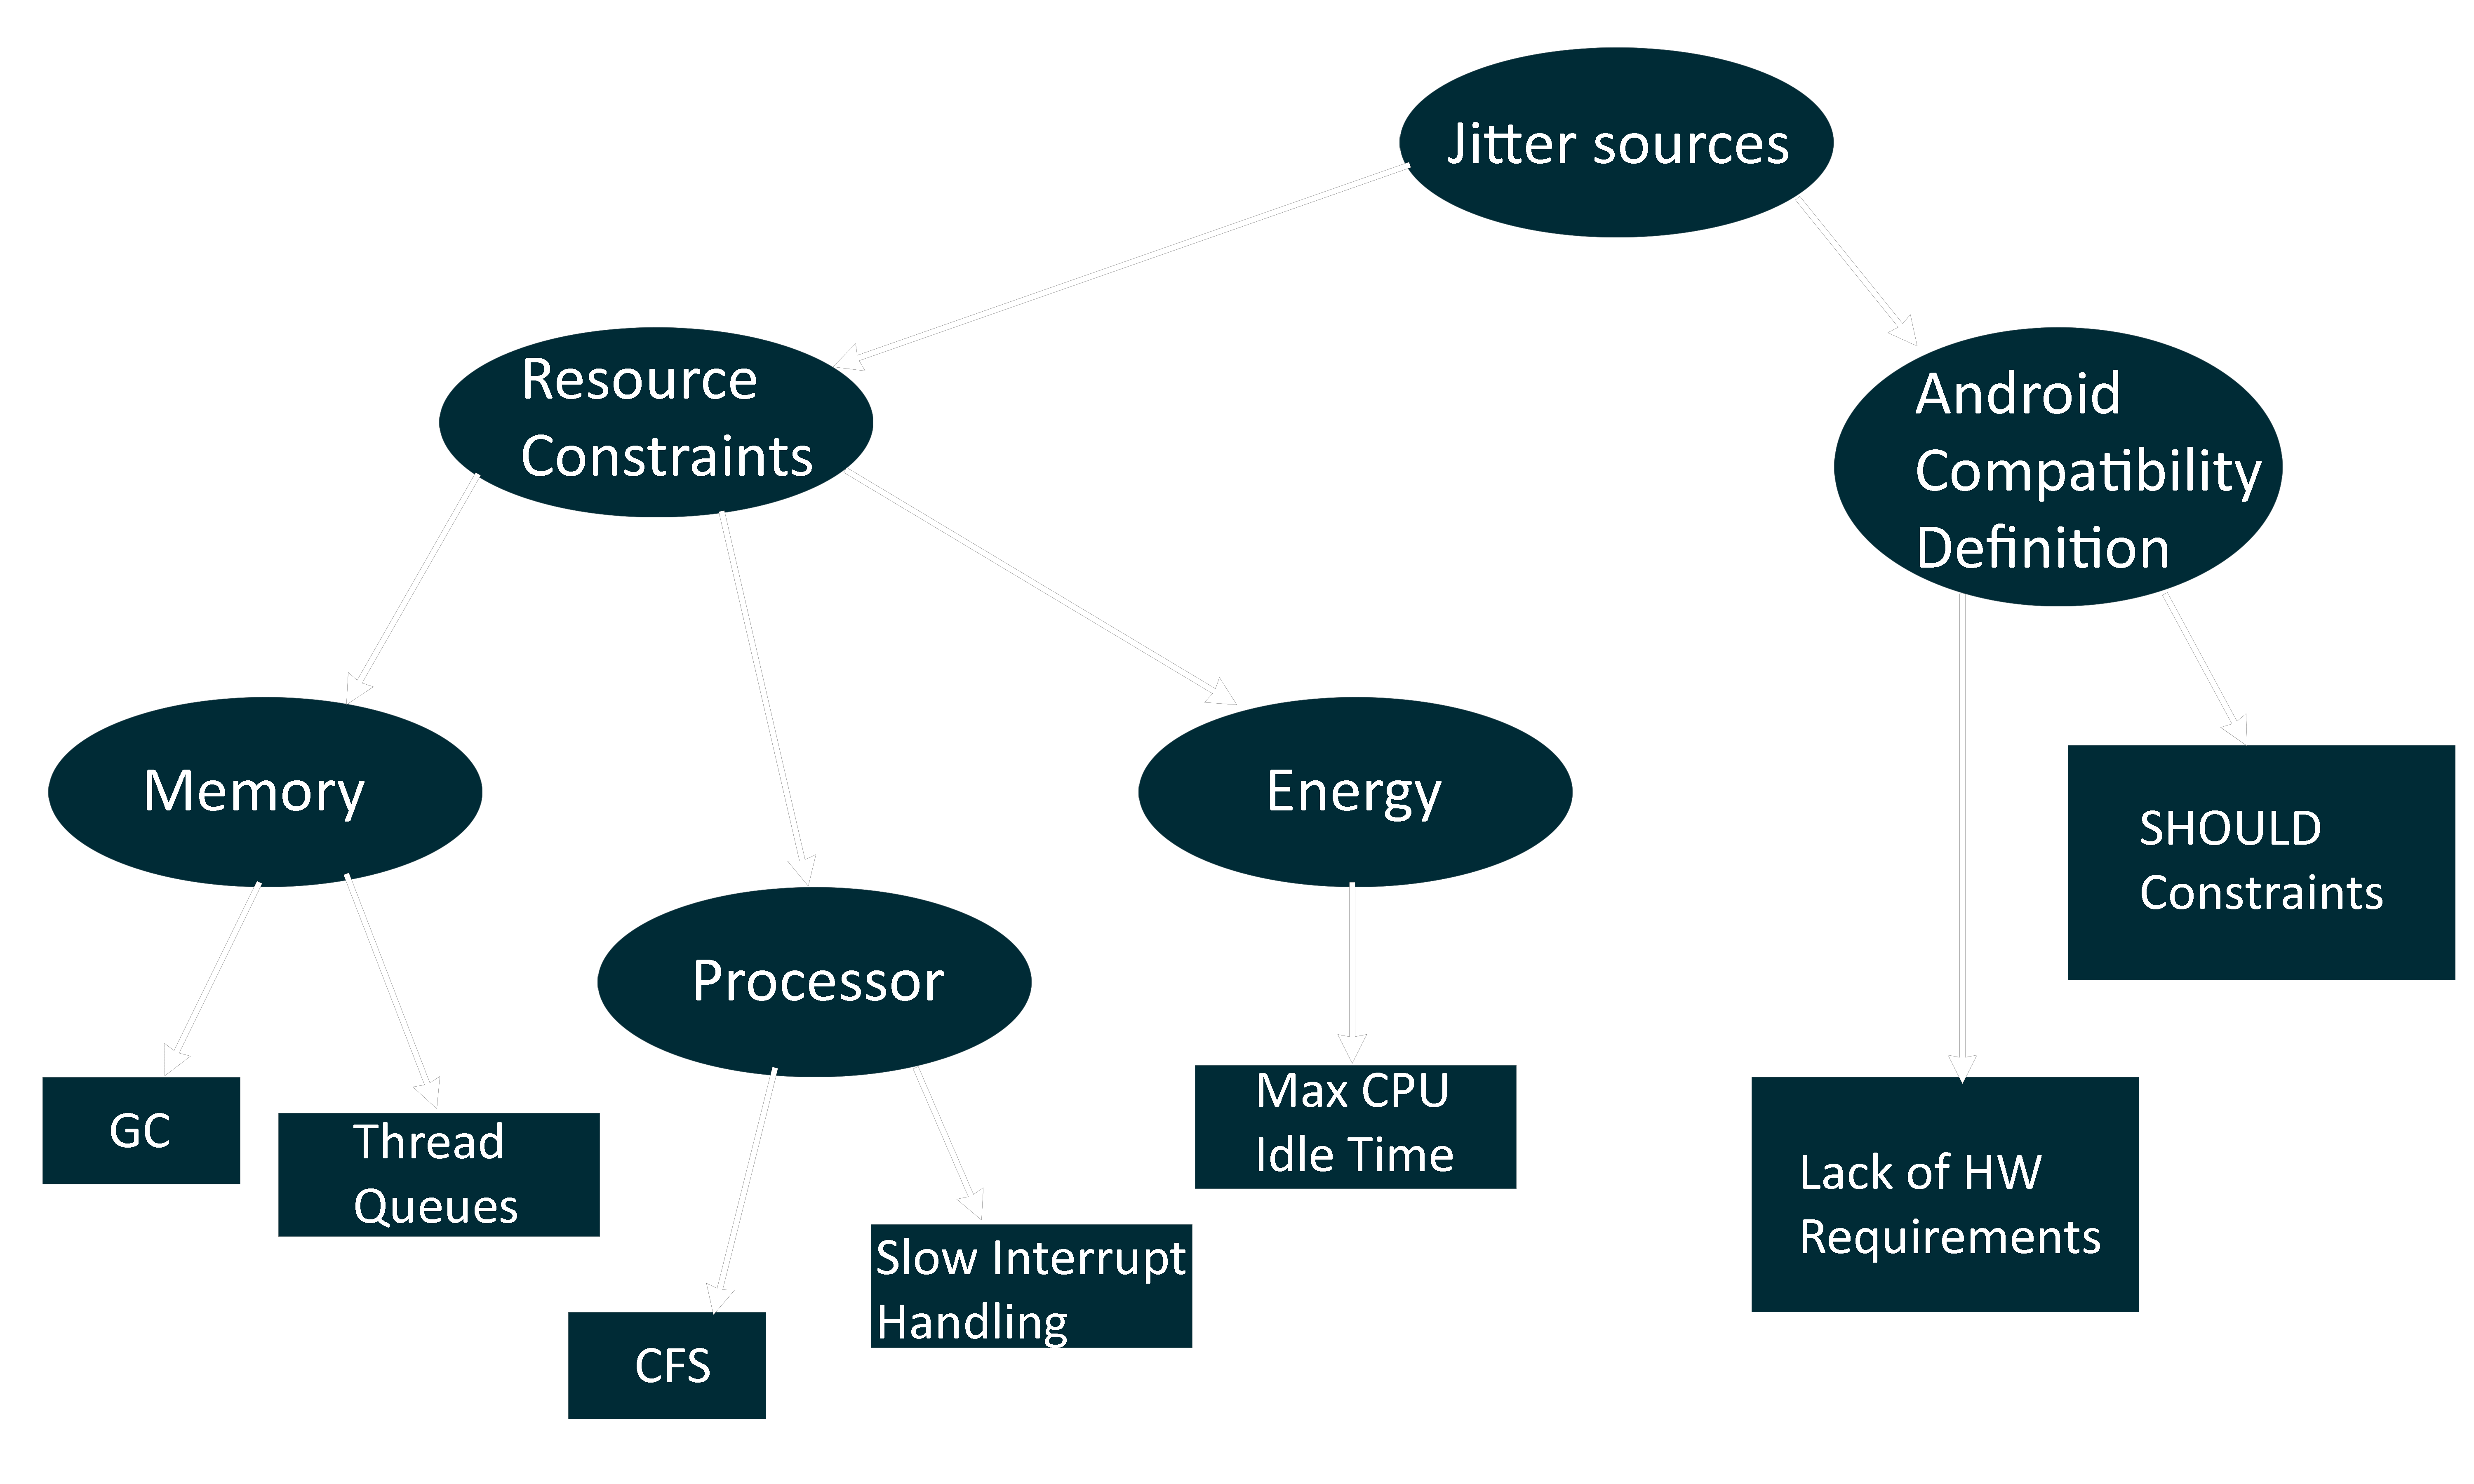
\includegraphics[scale=0.055]{androidJitter}
\end{frame}
\subsection{Isolamento di una CPU}
\begin{frame}{Isolamento di una CPU}
	\vspace{-10px}
	\centering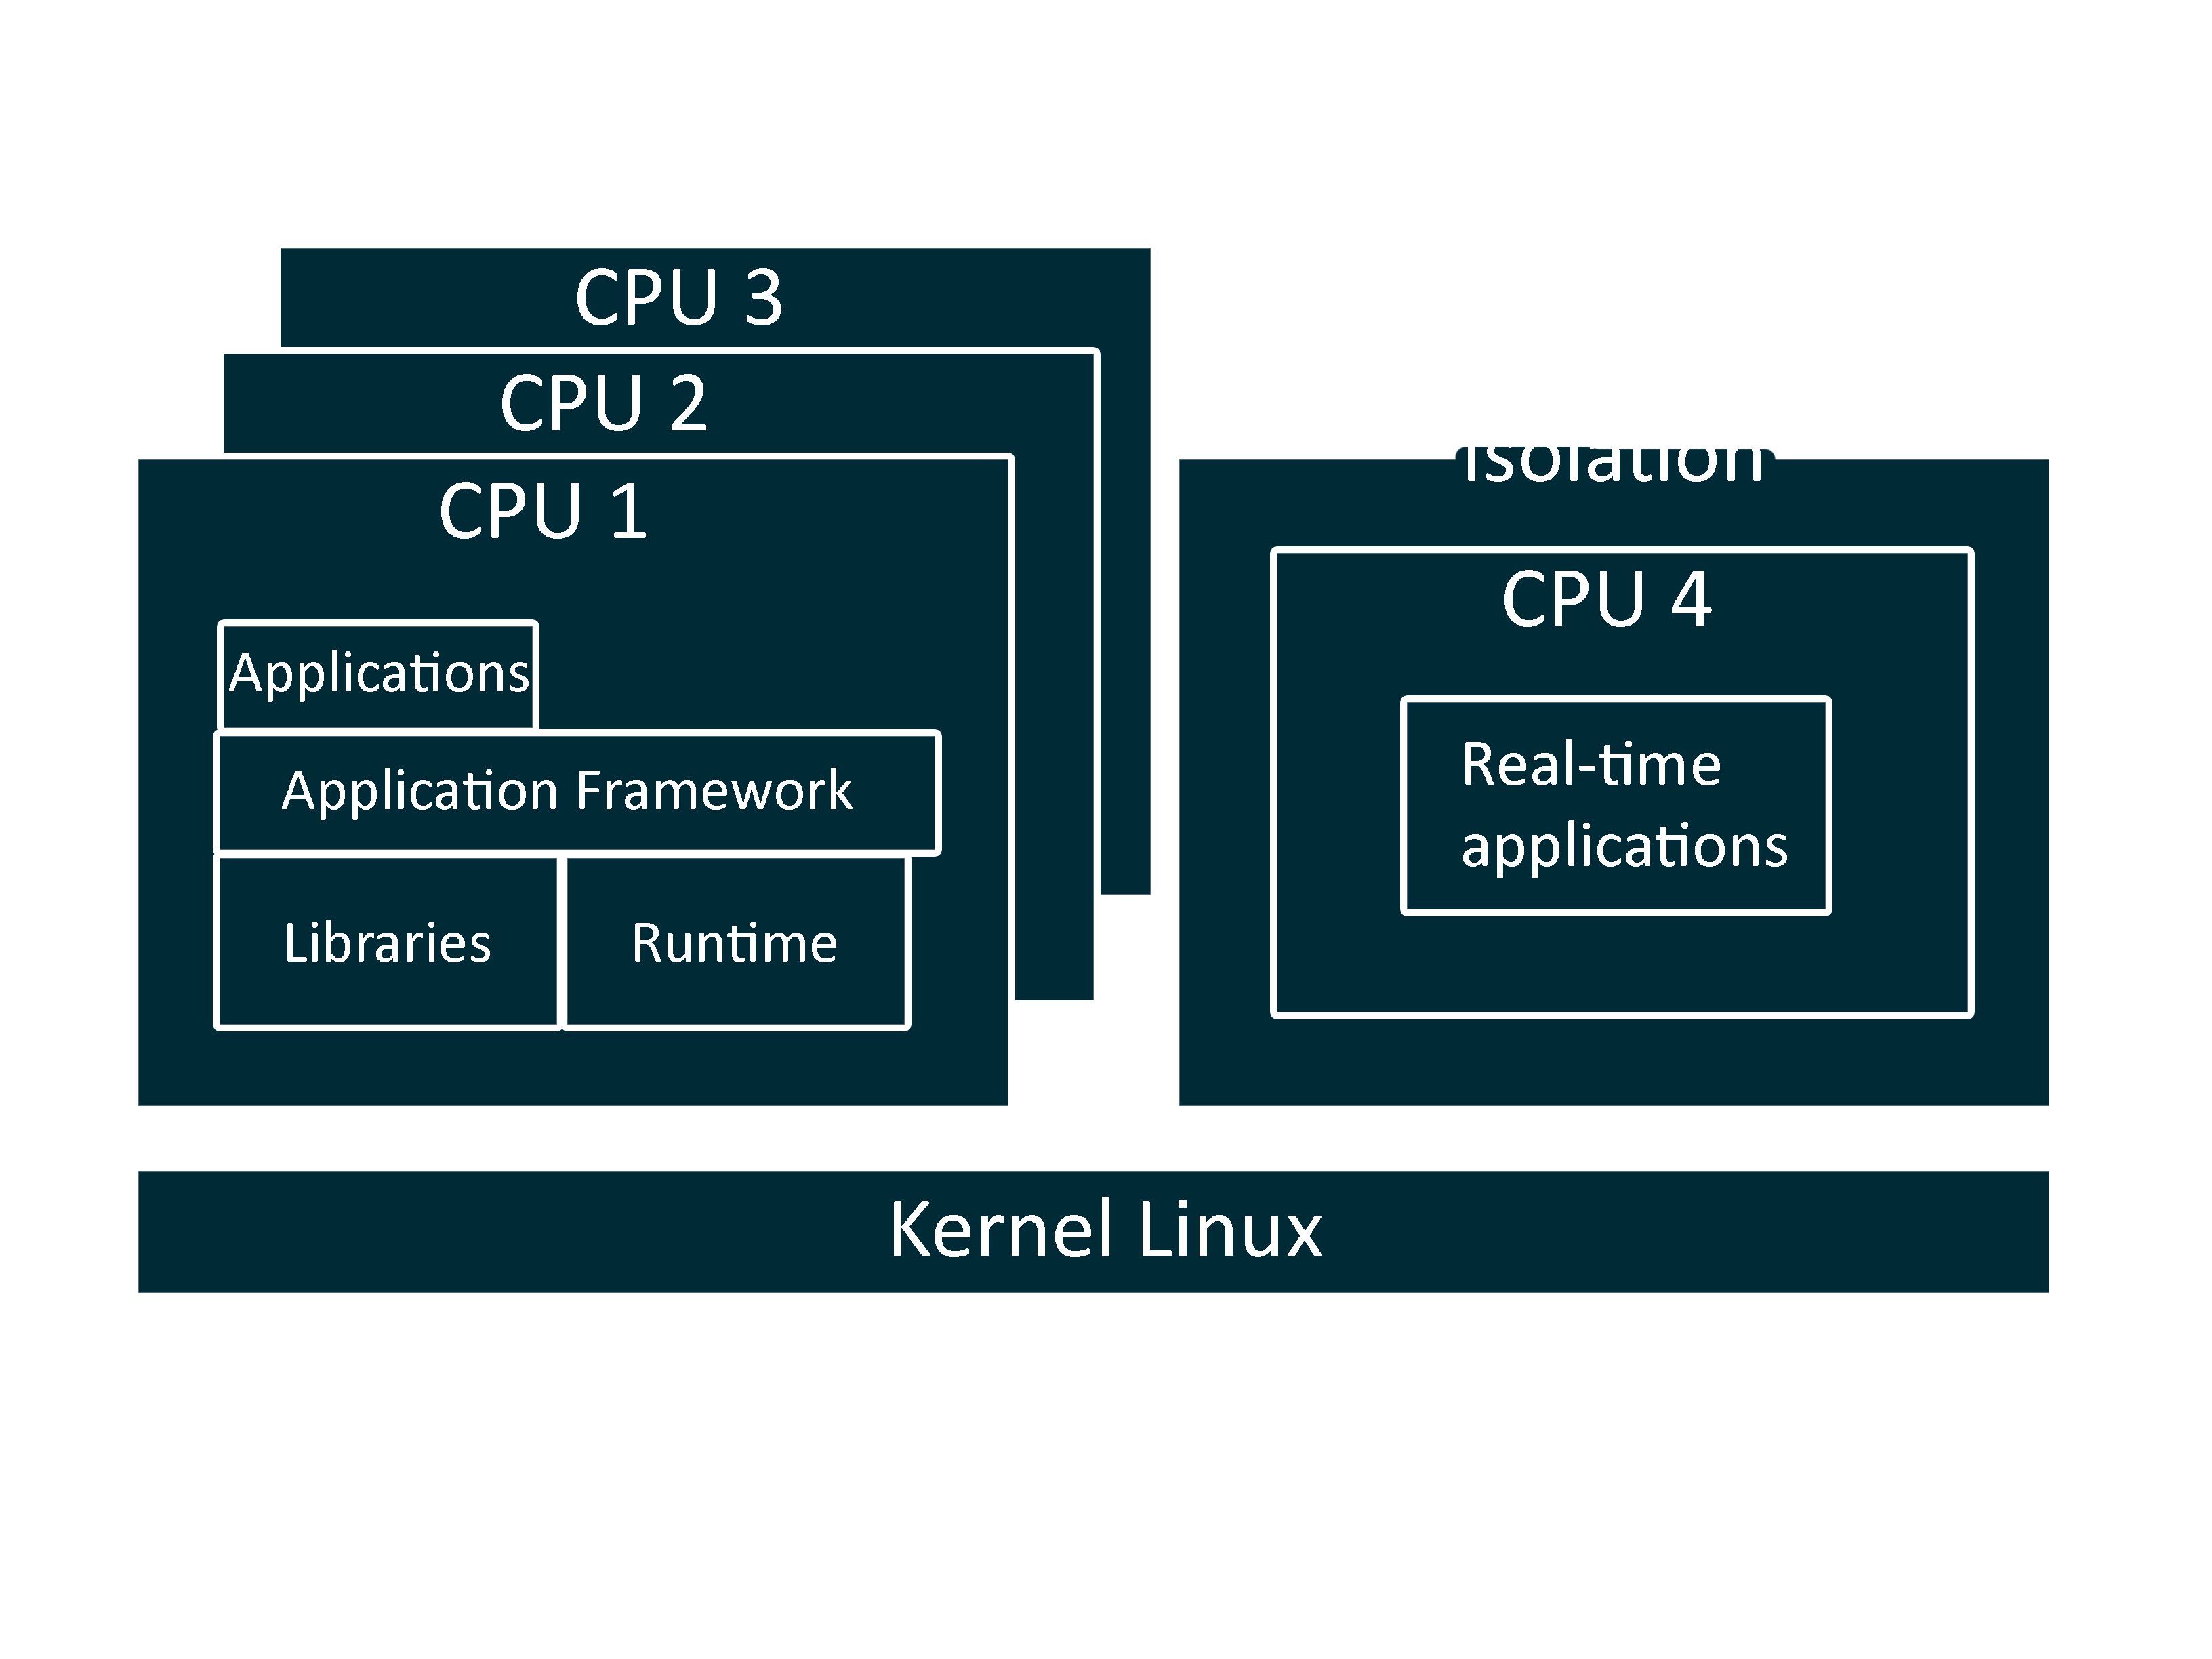
\includegraphics[scale=0.1]{cpuisol}
\end{frame}
\begin{frame}{Isolamento di una CPU - Azioni}
	\begin{itemize}
		\item Dividere le CPU in due gruppi
		\begin{itemize}
			\item \texttt{CONFIG\_CPUSETS}
		\end{itemize}
		\item Gestire l'affinità interruzioni-CPU 
		\begin{itemize}
			\item \texttt{smp affinity}
		\end{itemize}
		\item Scheduling con \texttt{SCHED\_FIFO}
		\item Rendere il kernel prerilasciabile 
		\begin{itemize}
			\item \texttt{CONFIG\_PREEMPT}
		\end{itemize}
		\item Fissare la frequenza della CPU
		\item Inibire il risparmio energetico
	\end{itemize}
\end{frame}
\begin{frame}{Isolamento di una CPU - Valutazione}
	Vantaggi
	\begin{itemize}
		\item[+] Riduzione del jitter
		\begin{itemize}
			\item Una CPU viene ``dedicata'' ad un utilizzo RT
		\end{itemize}
		\item[+] Nessuna modifica al kernel
		\begin{itemize}
			\item Ma alcune limitazioni del kernel Linux restano
		\end{itemize}
		\item[+] Nessuna modifica dell'architettura
	\end{itemize}
	\vspace{10px}
	Svantaggi
	\begin{itemize}
		\item[-] Nessun supporto allo scambio di messaggi
		\item[-] Impedisce il risparmio energetico
		\begin{itemize}
			\item In contrasto con le direttive CDD
		\end{itemize}
		\item[-] Adatto solo ad applicazioni soft real-time
		\begin{itemize}
			\item Considerando che le fonti di jitter non sono annulate
		\end{itemize}
	\end{itemize}
\end{frame}

\section{RTDroid}
\begin{frame}{RTDroid - Architettura}
	\vspace{-10px}
	\only<1>{\centering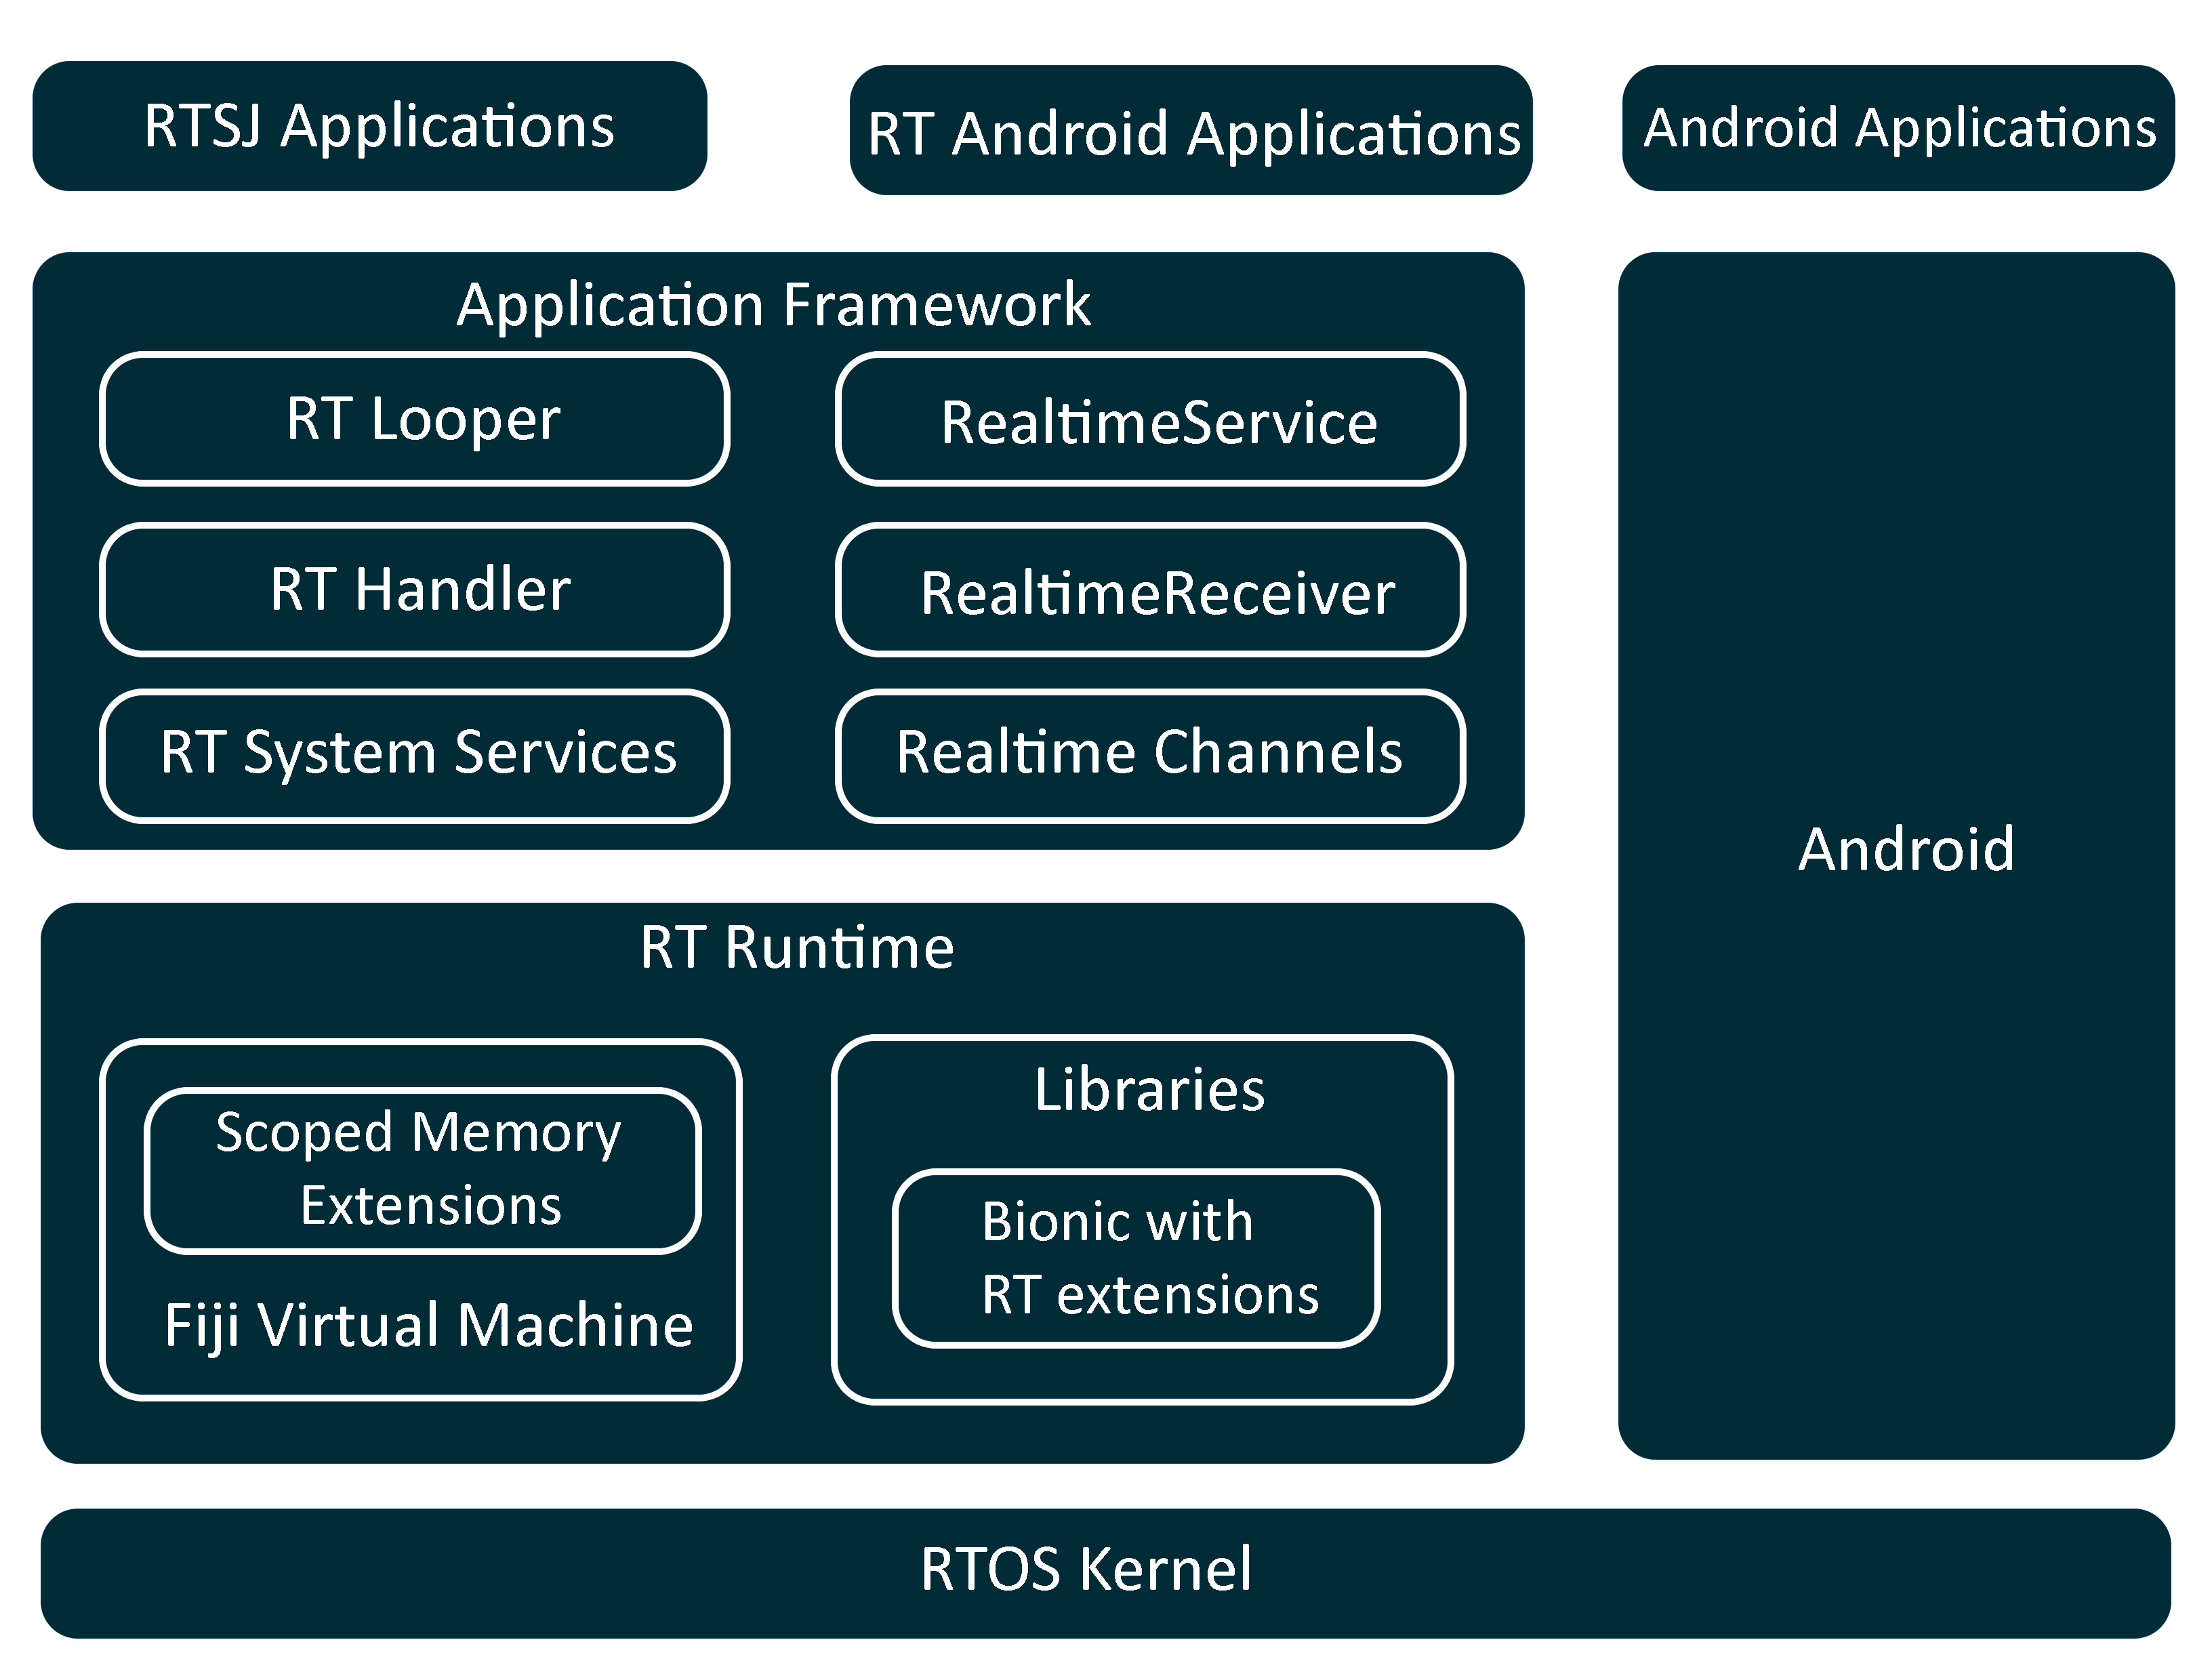
\includegraphics[scale=0.08]{RTDroid}}
	
	\only<2>{\centering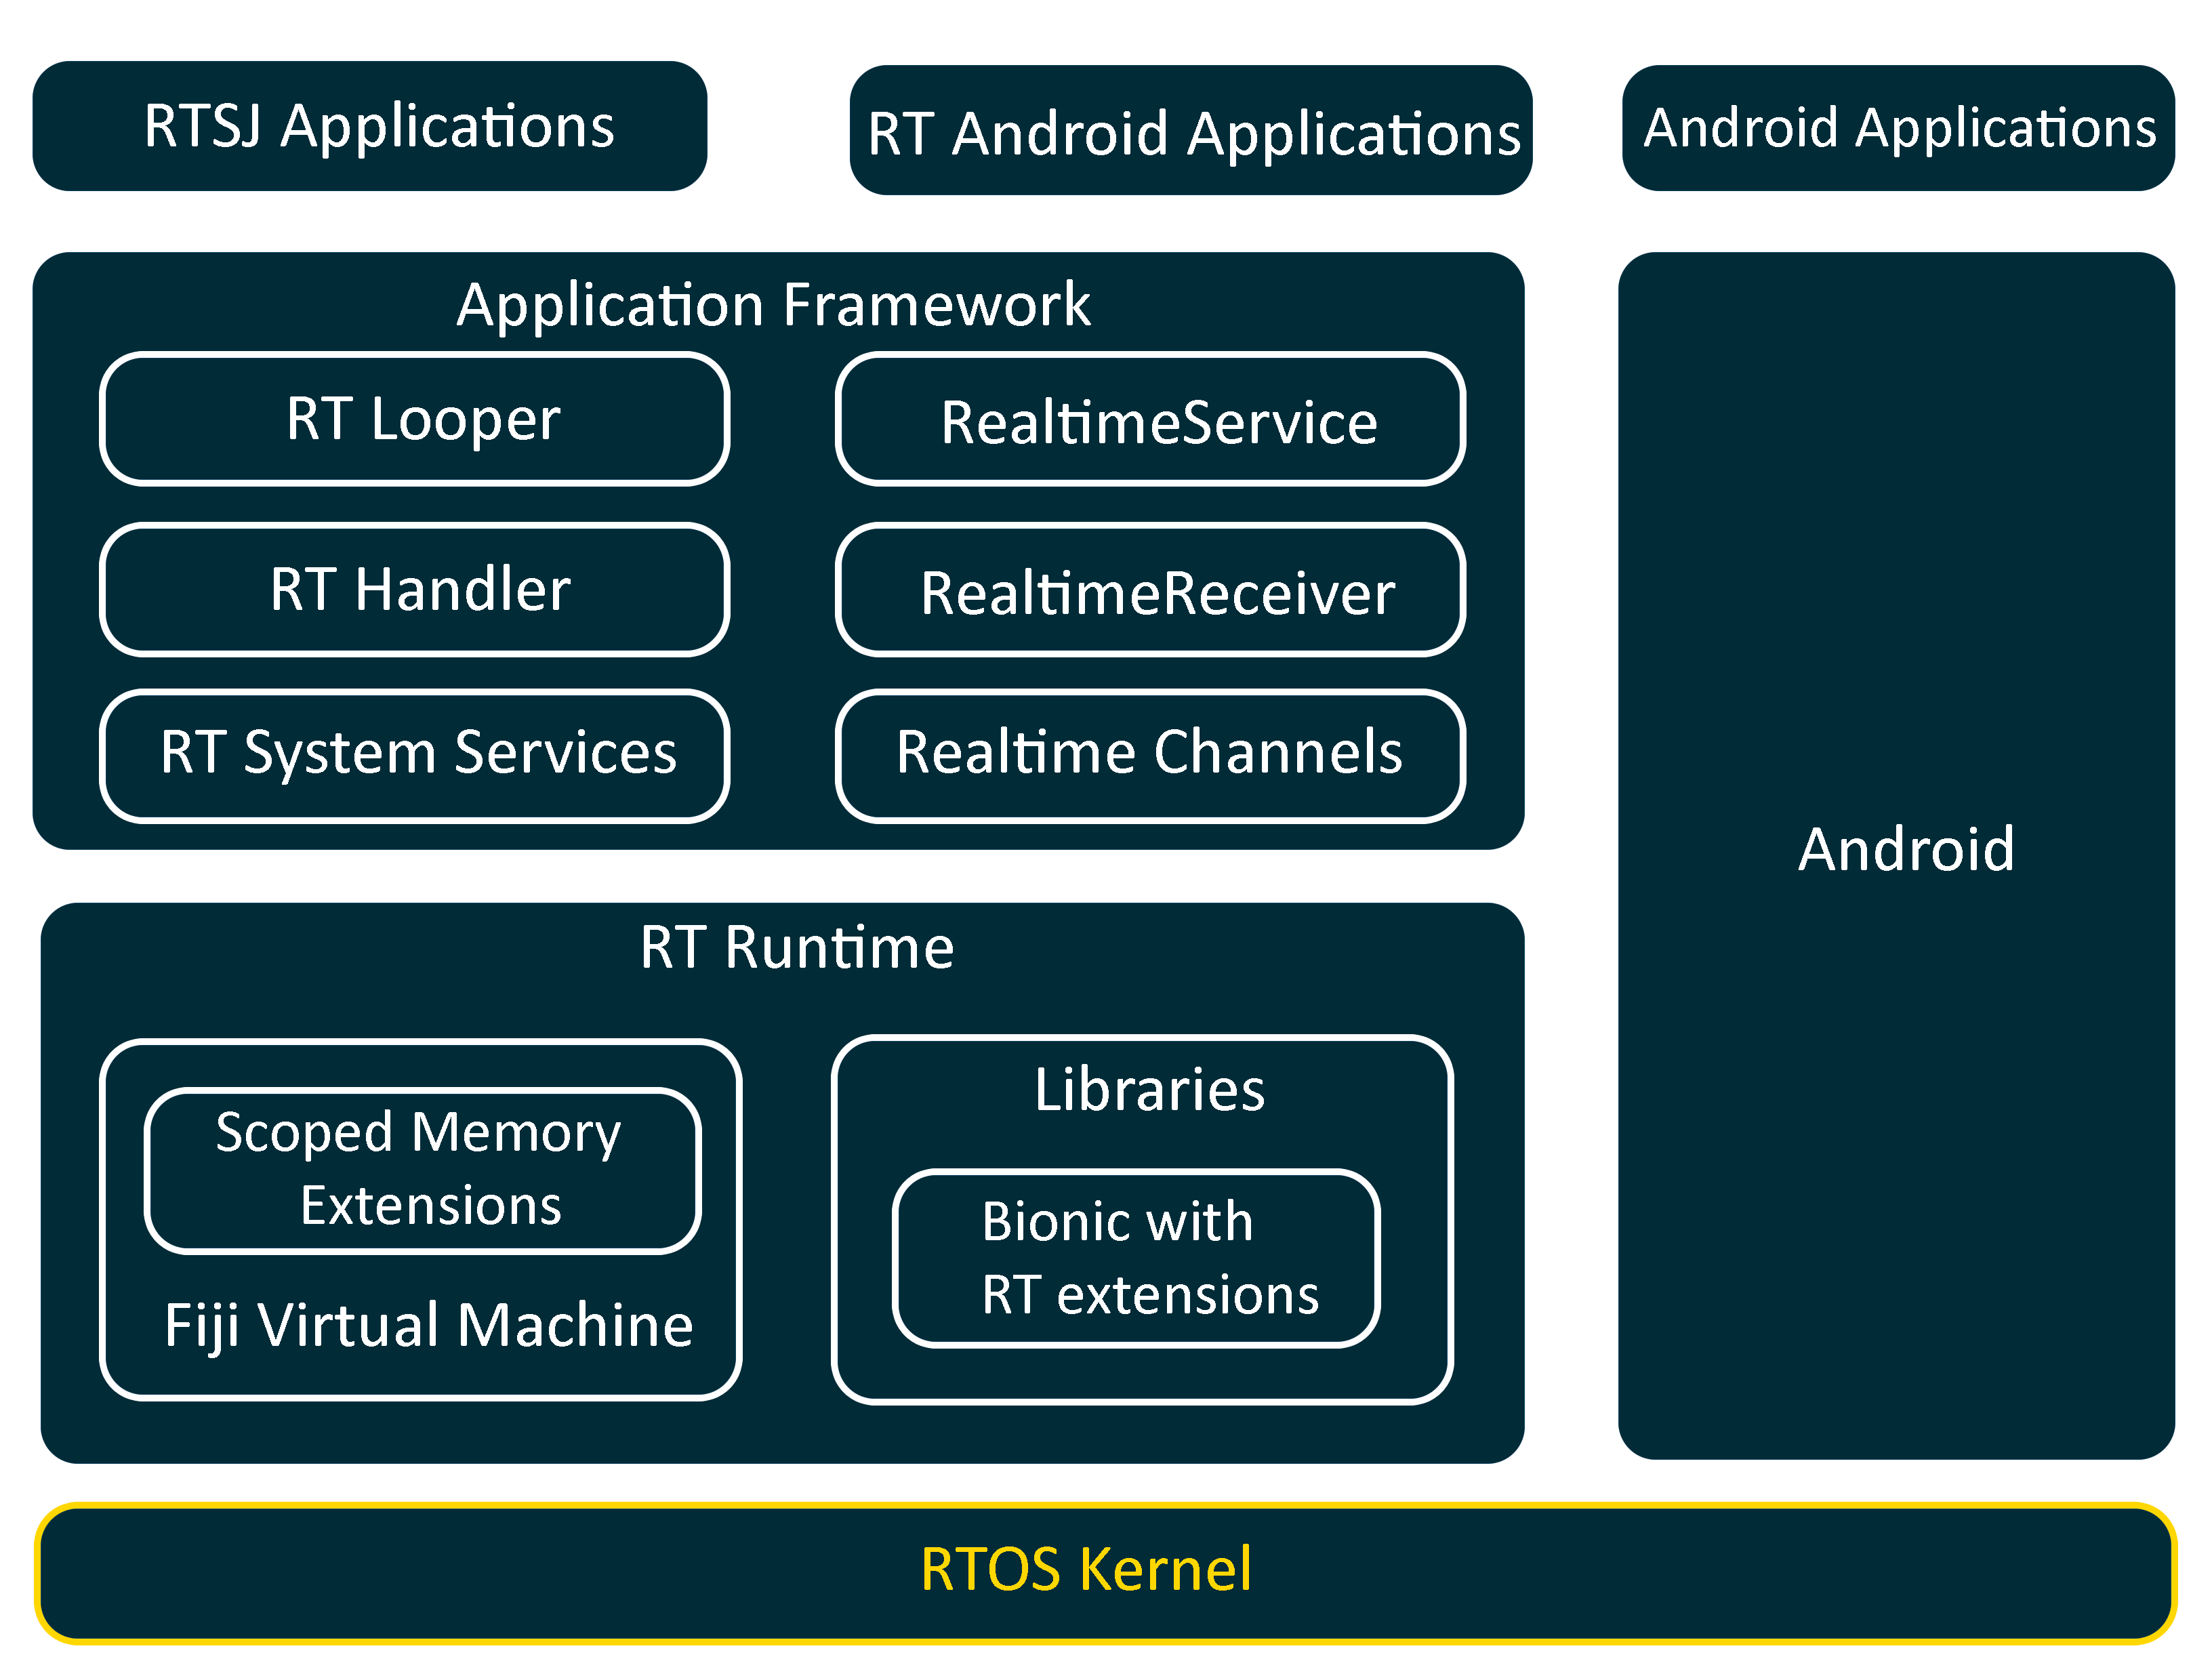
\includegraphics[scale=0.08]{RTDroidGoldKernel}}
	
	\only<3>{\centering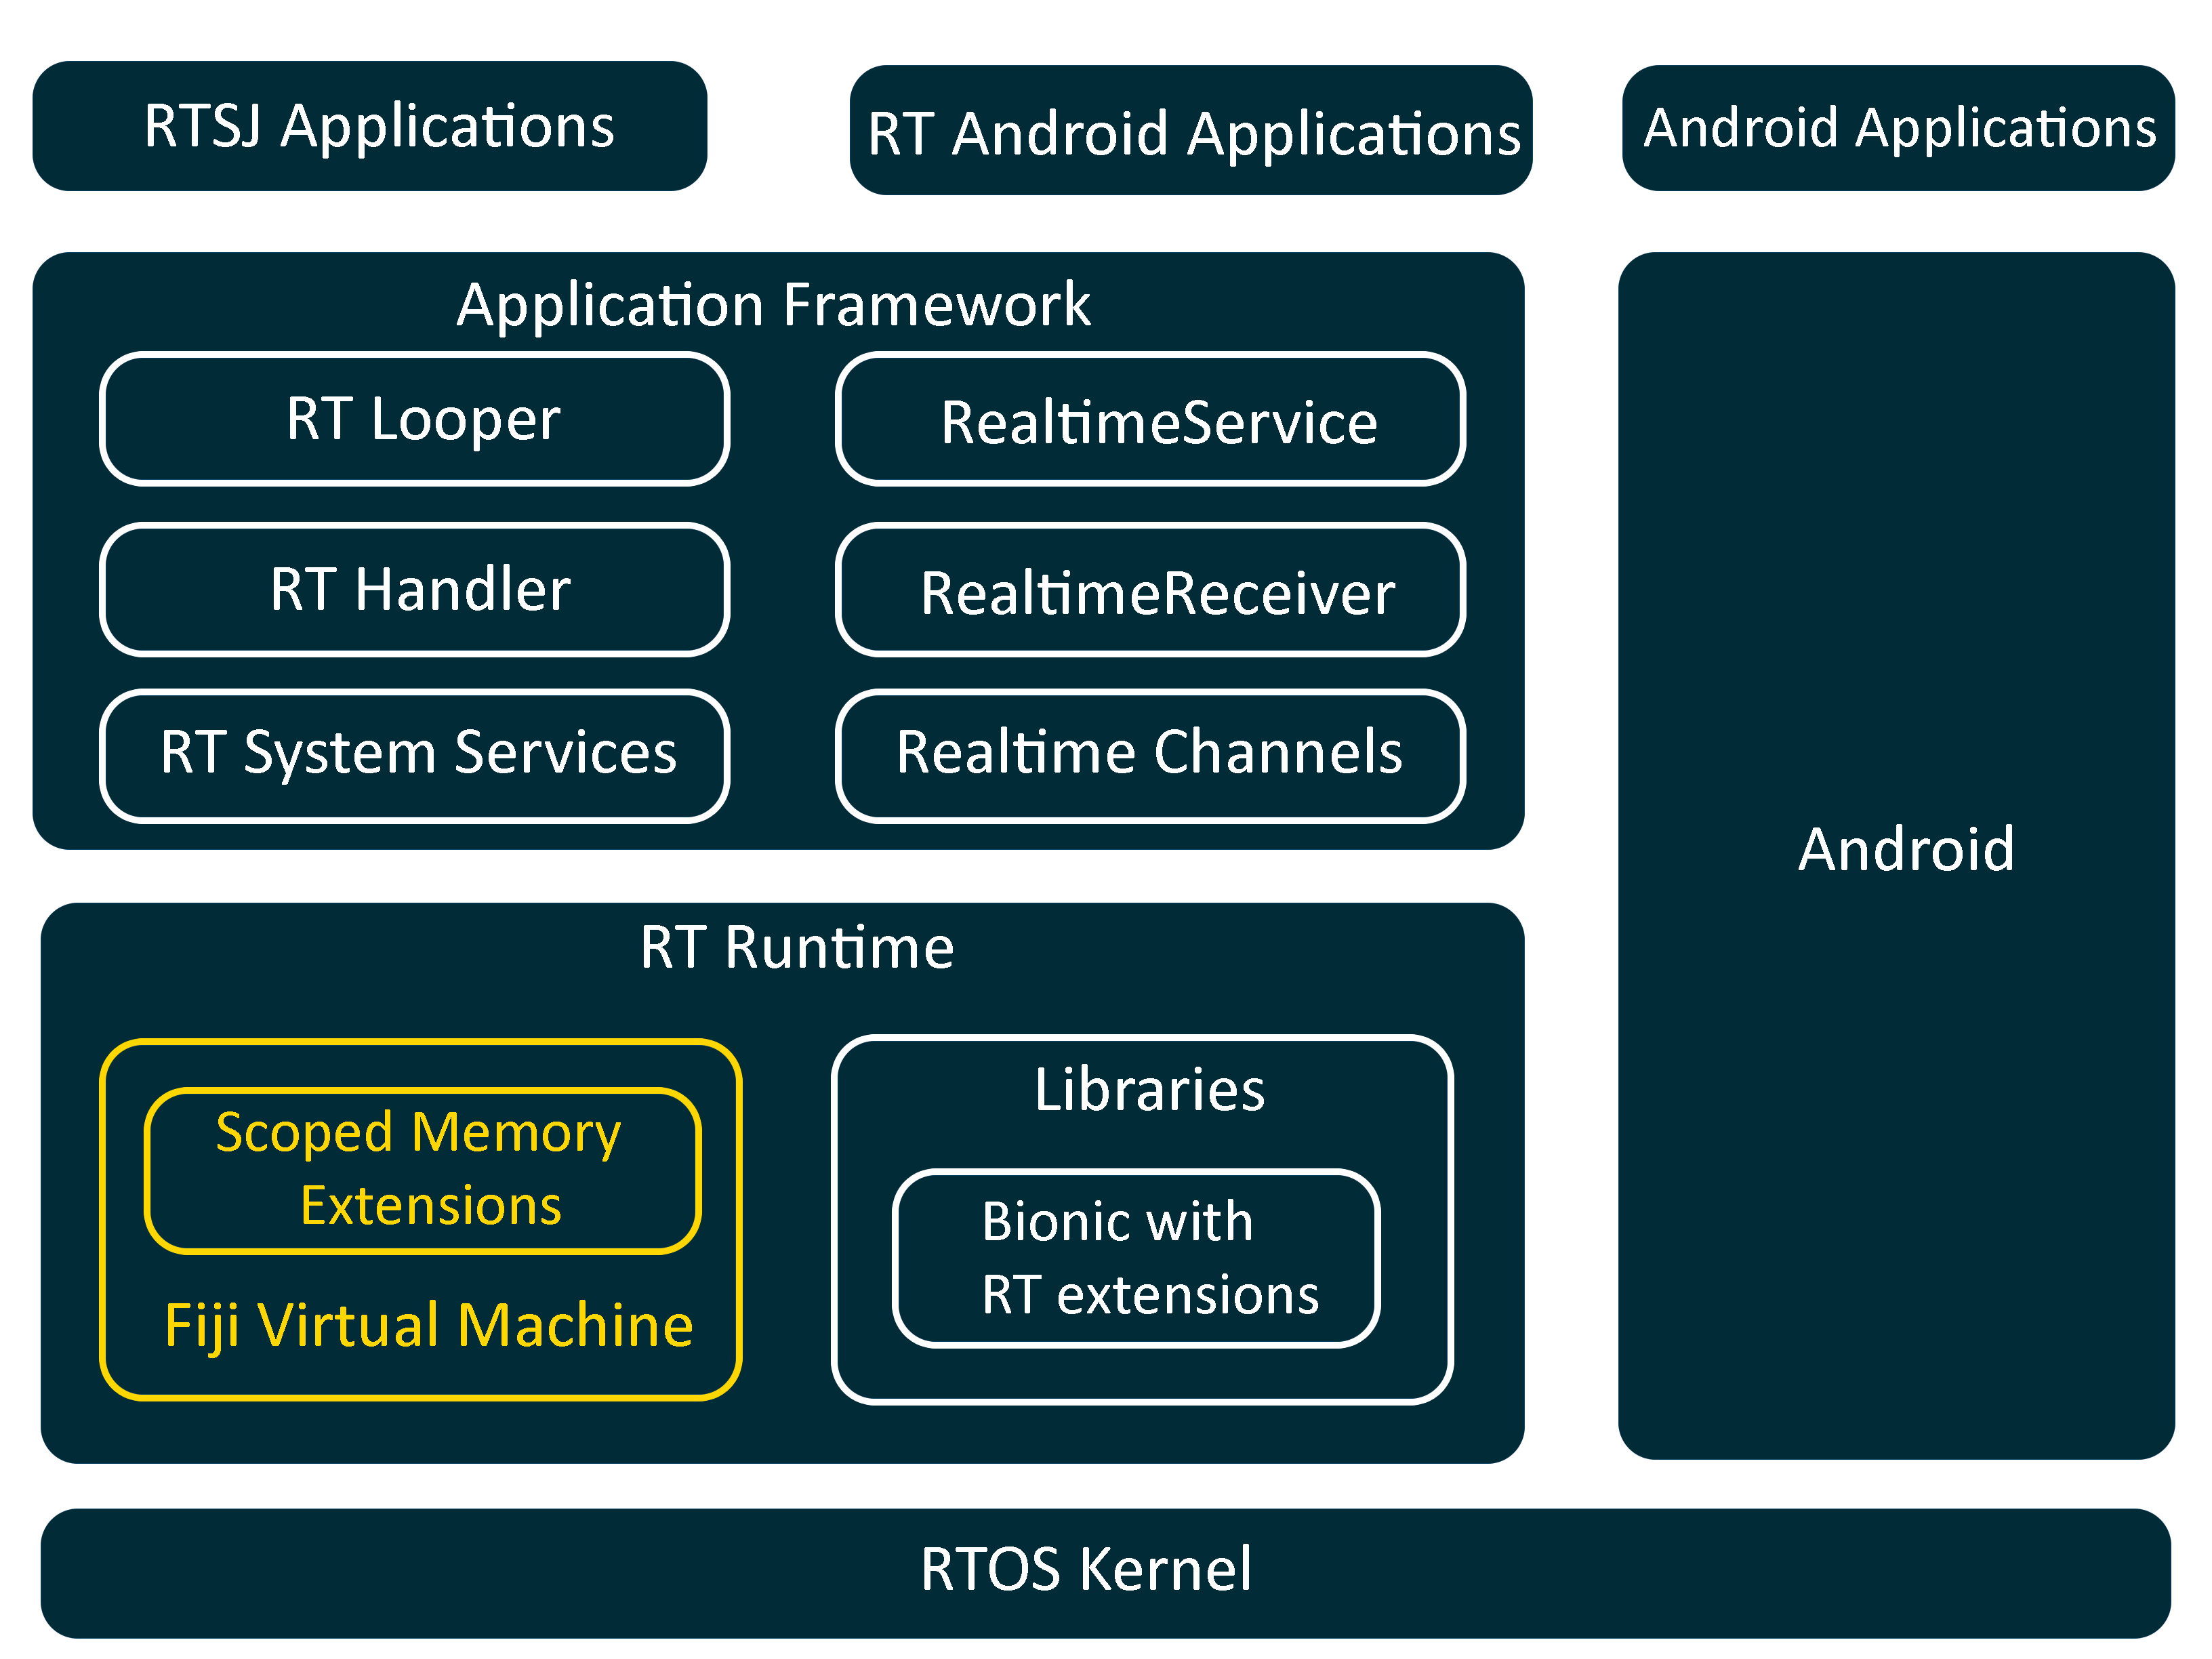
\includegraphics[scale=0.08]{RTDroidGoldJVM}}
	
	\only<4>{\centering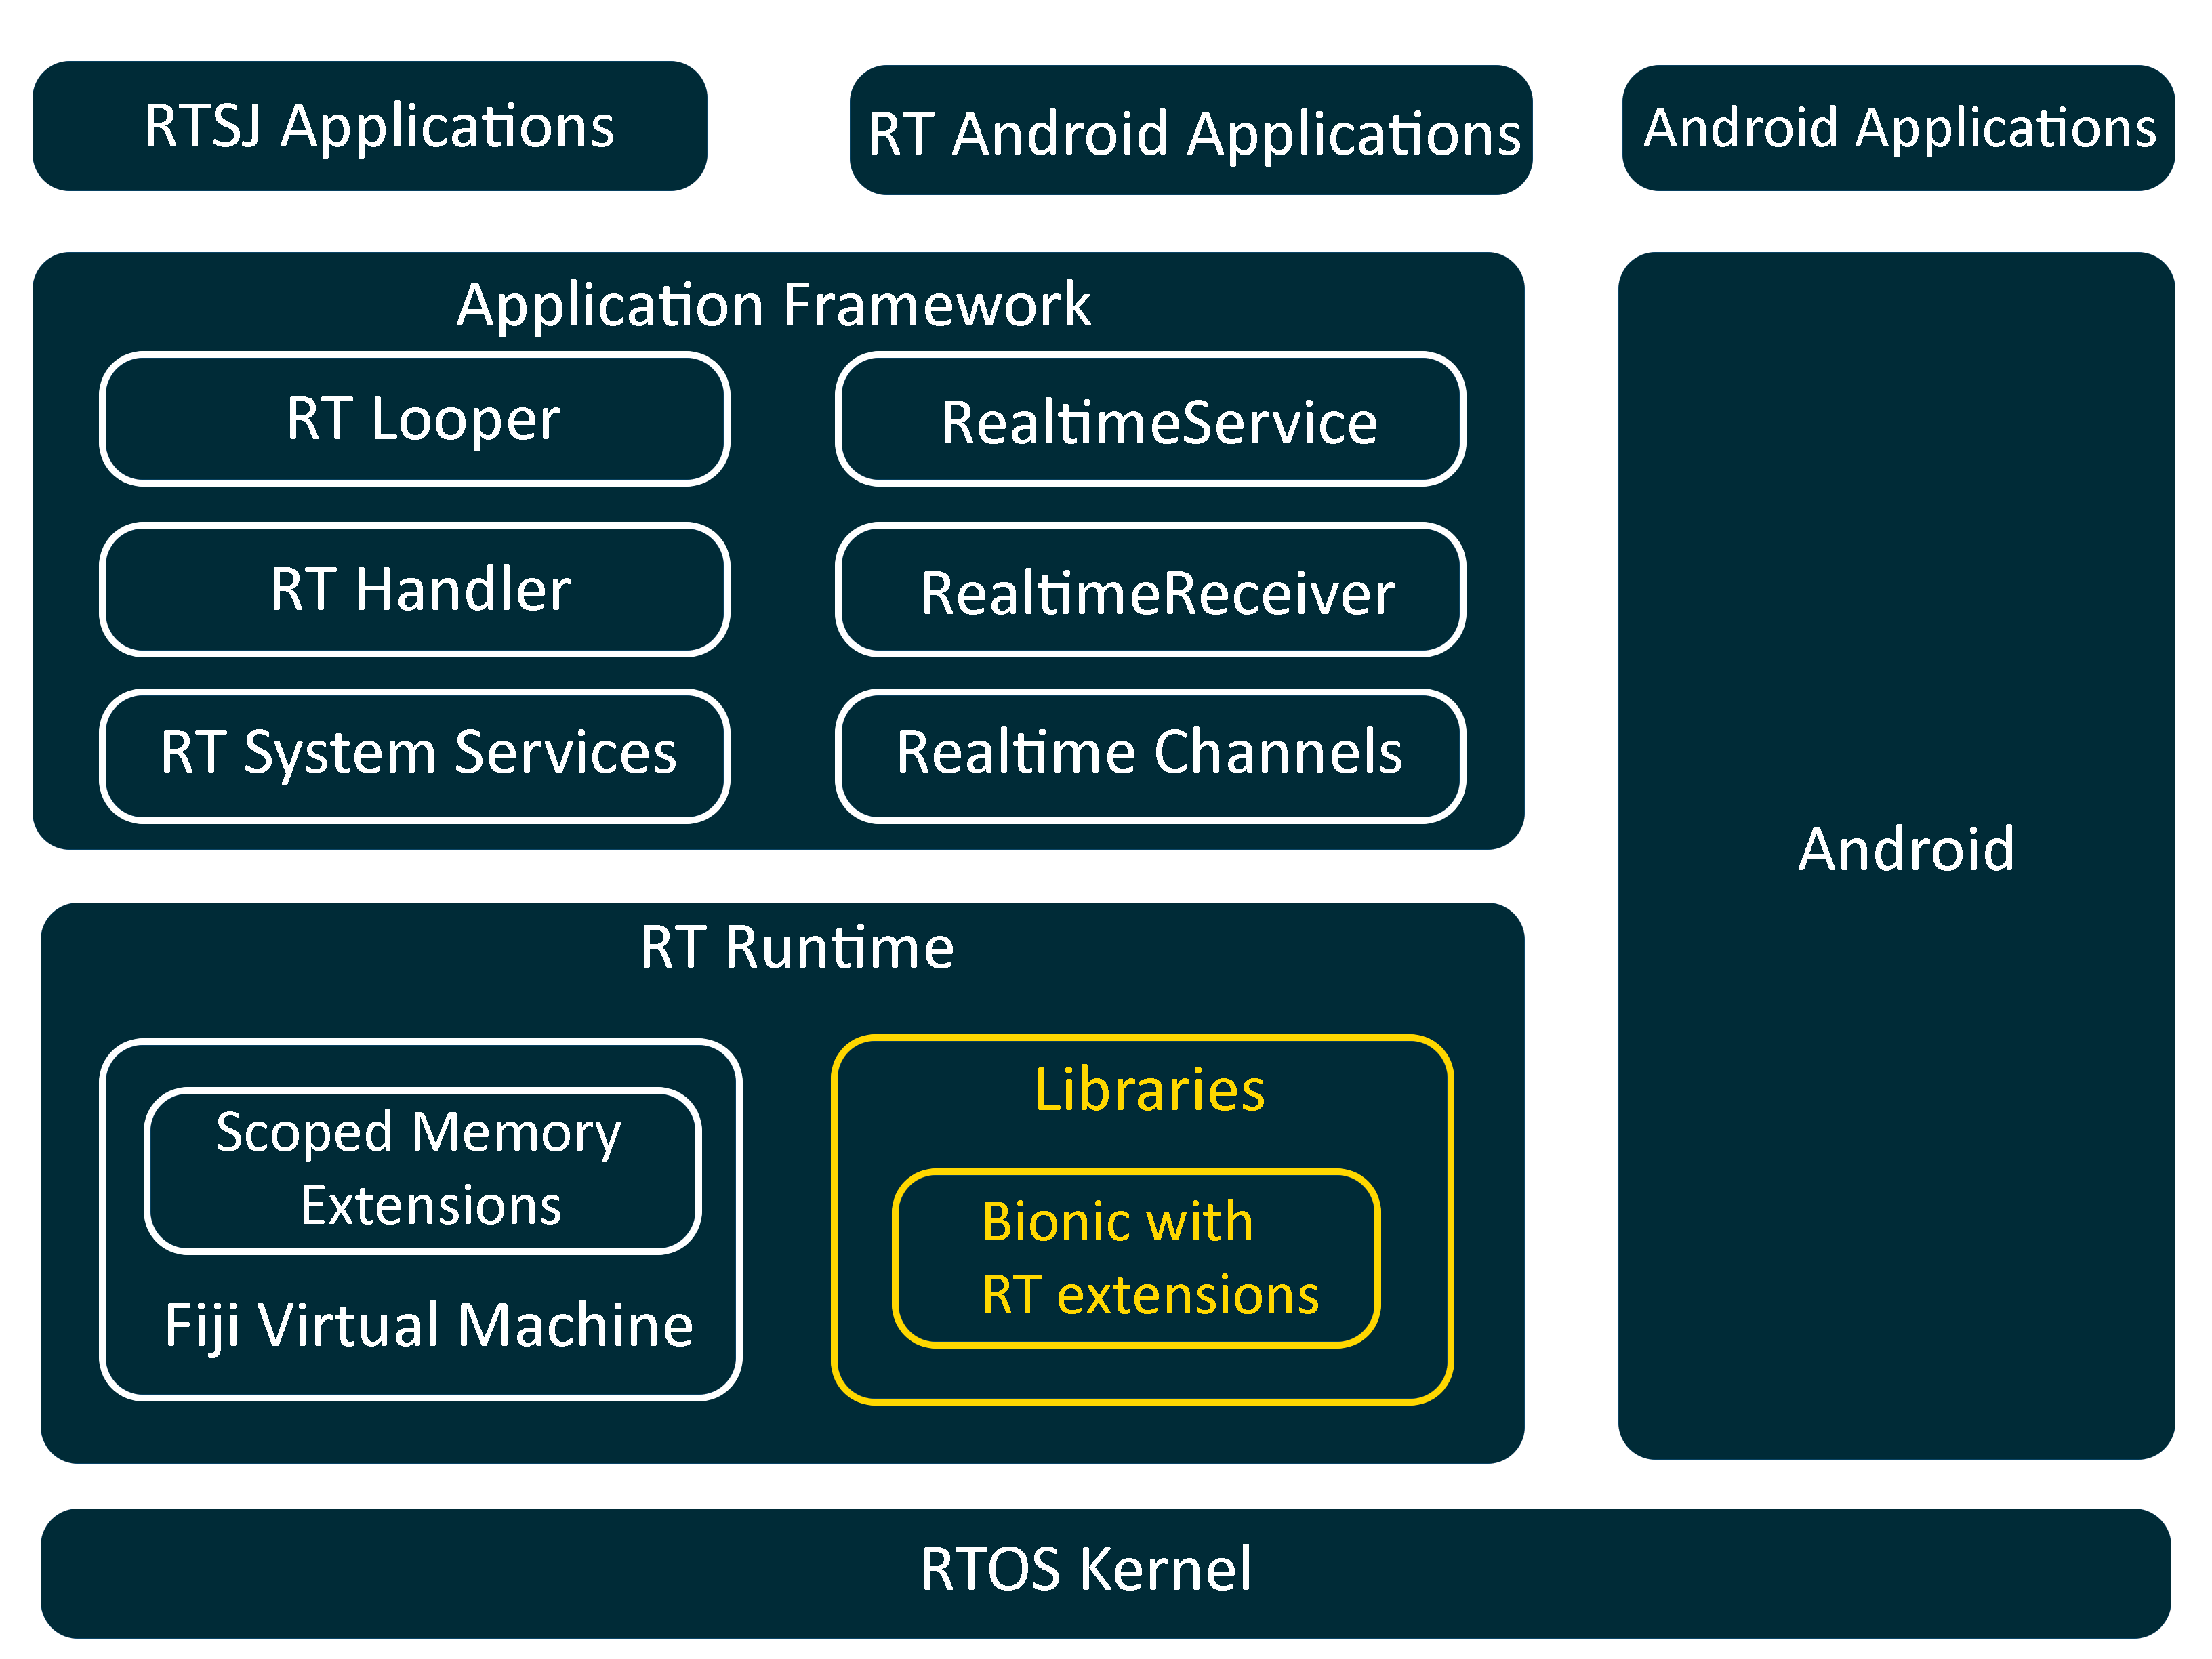
\includegraphics[scale=0.08]{RTDroidGoldLib}}
	
	\only<5>{\centering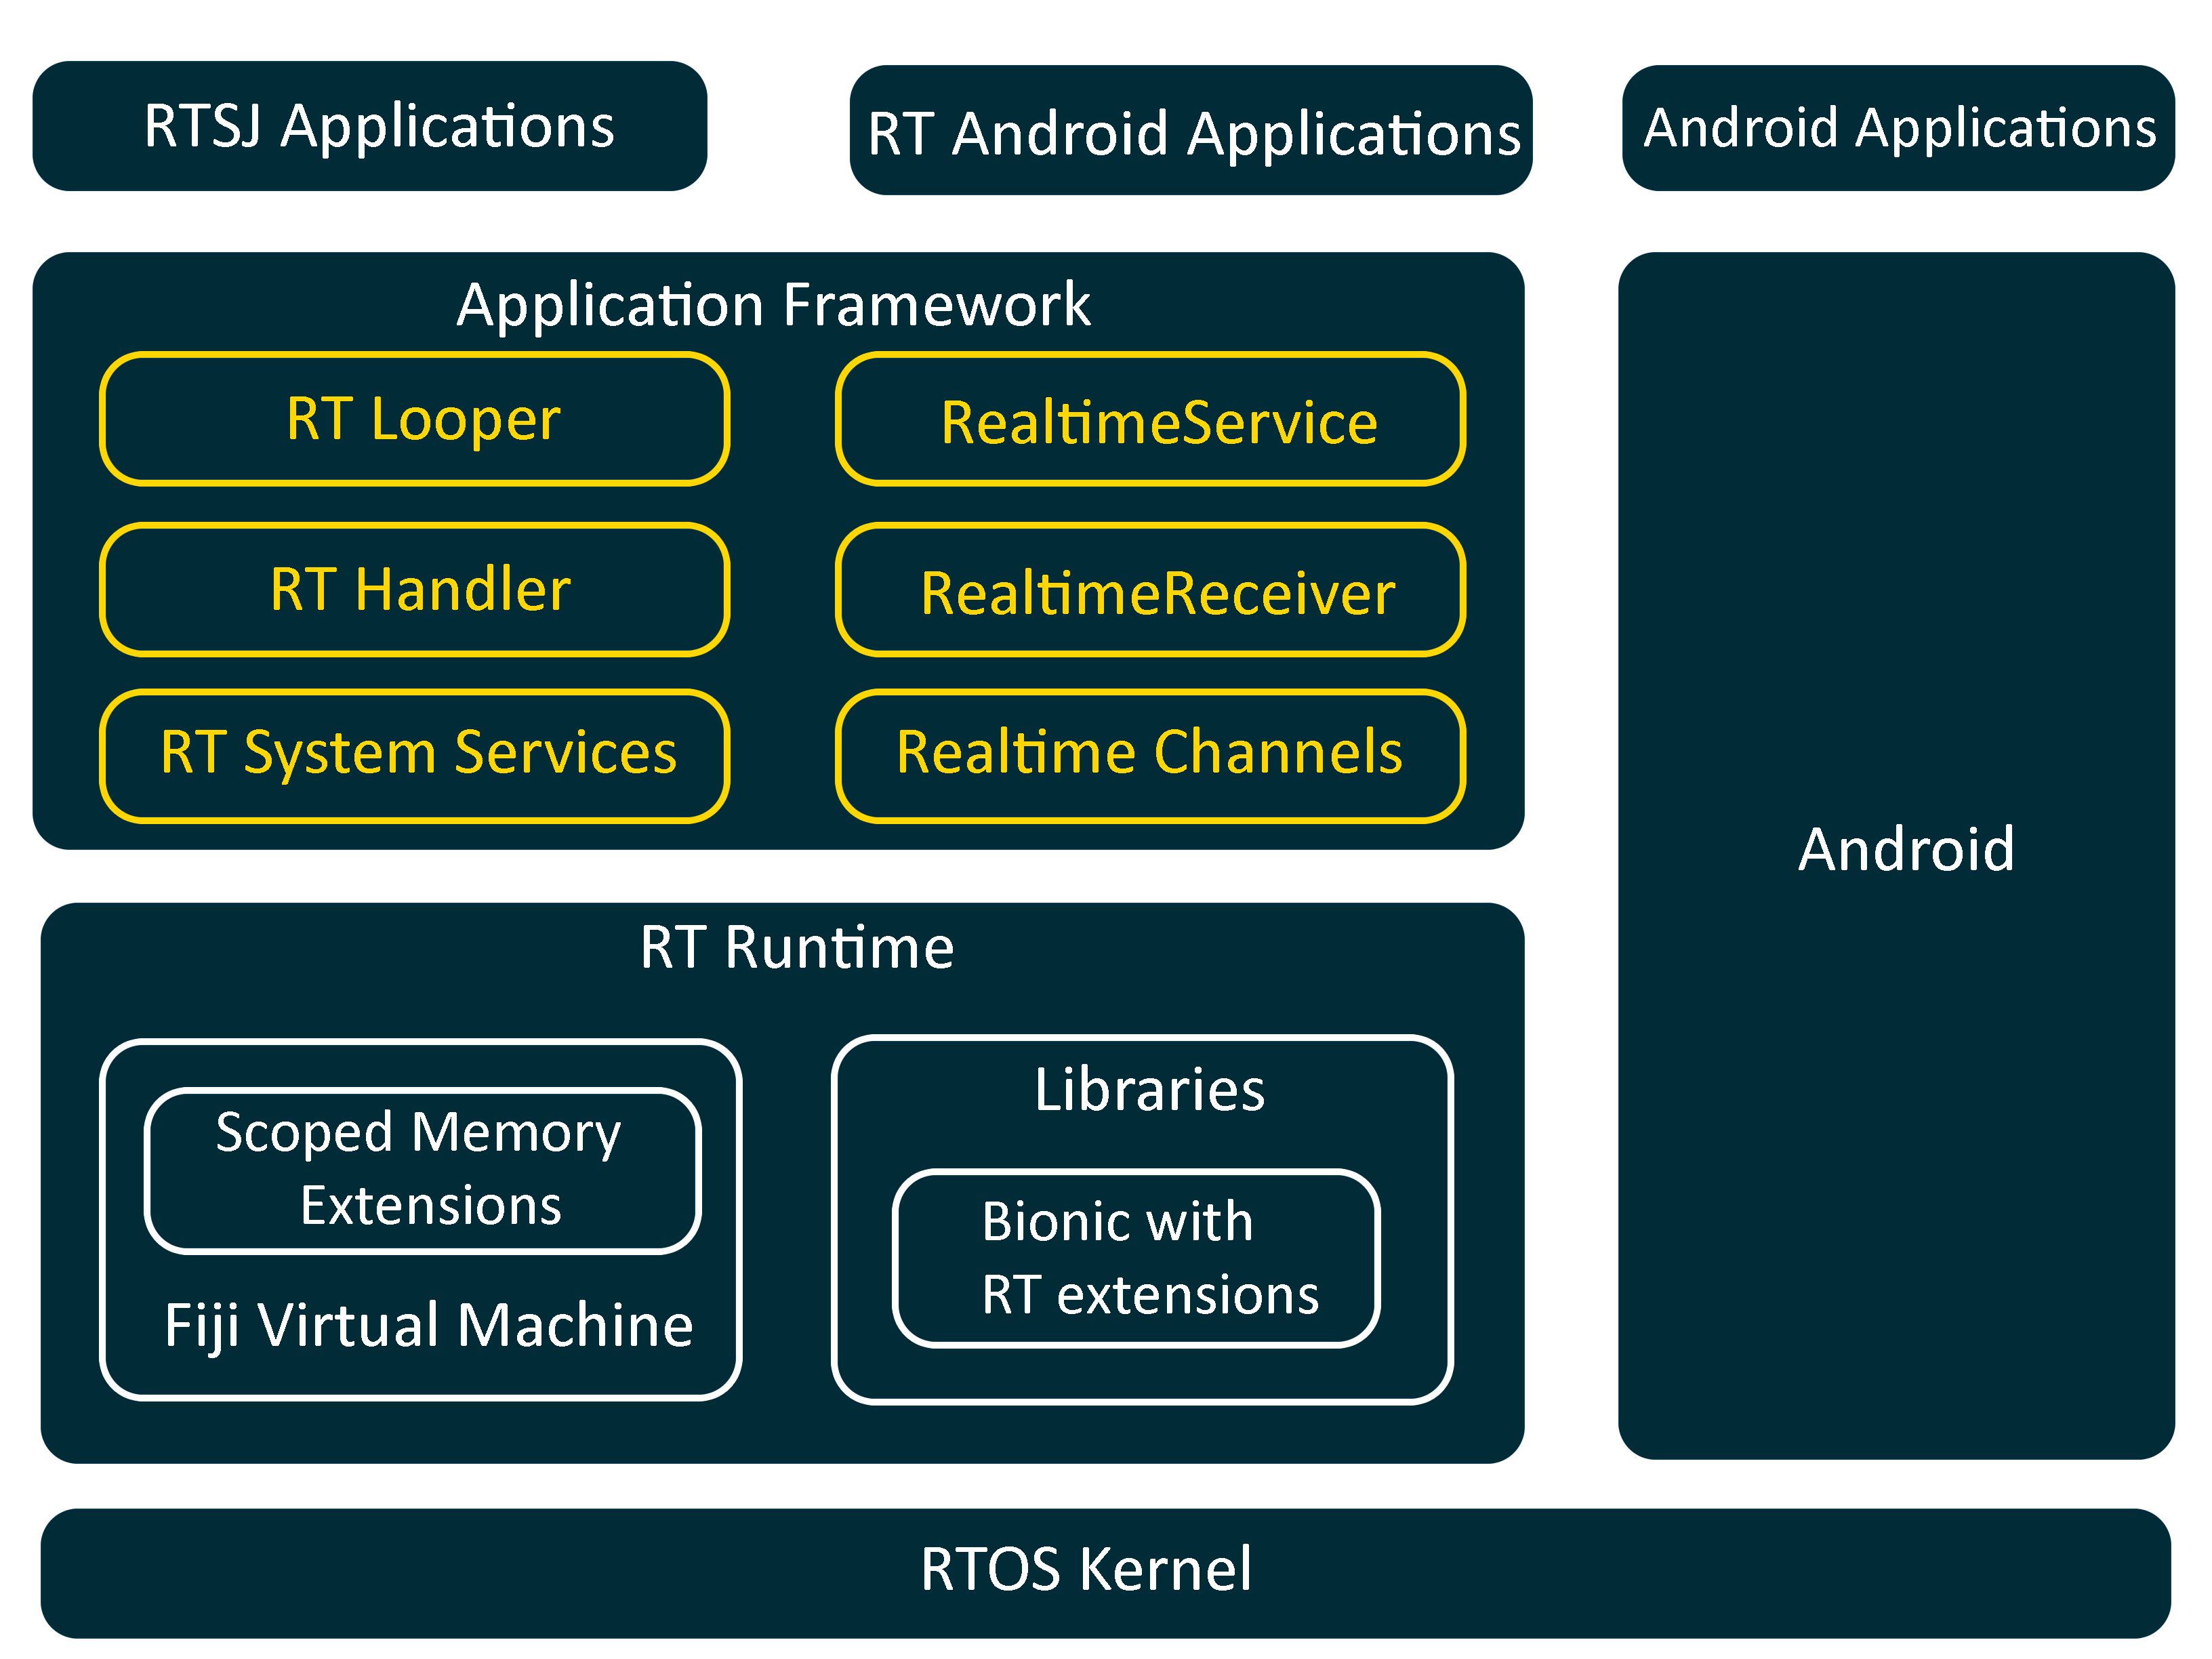
\includegraphics[scale=0.08]{RTDroidGoldRTComp}}
\end{frame}
\subsection{Componenti di base}
\section{Fiji VM}
I linguaggi più utilizzati, in genere, per sistemi real-time sono Ada e C (per i più coraggiosi C++). Tuttavia la complessità e la dimensione crescente del codice, unita alla disponibilità di tanti programmatori ben addestrati hanno portato fatto crescere l'interesse verso l'utilizzo di Java. Inoltre, dato che le applicazioni Android sono generalmente scritte in Java, per poter utilizzare quei dispositivi in contesti con vincoli temporali è necessario avvicinare il mondo Java e quello real-time. Per farlo è necessario sviluppare un runtime, e una GC, che siano prevedibili e adatti all'utilizzo in sistemi con vincoli temporali stretti. La Fiji VM (fVM) ha esattamente questo scopo. Figura\ref{fig:fijiarch} mostra la sua architettura.
\begin{figure}
	\centering
	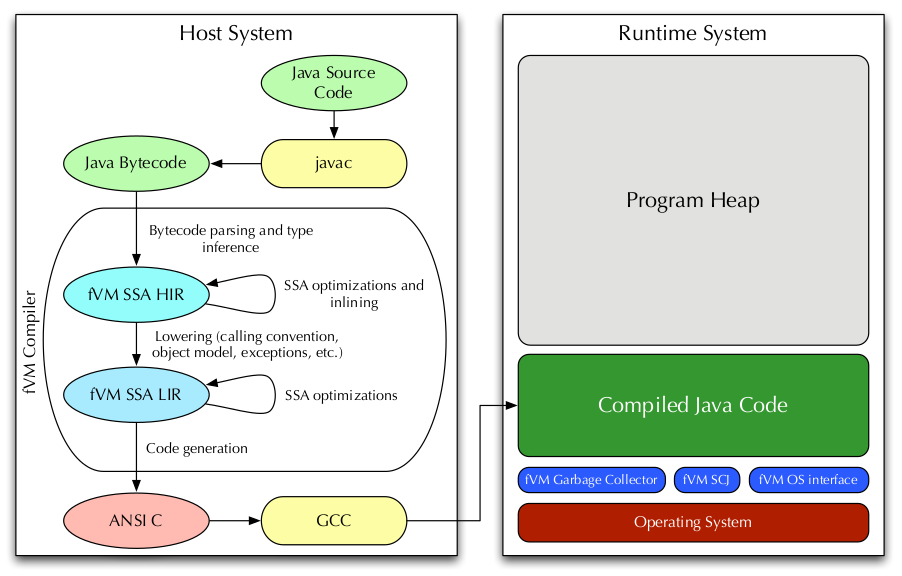
\includegraphics[width=0.9\linewidth]{fijiarch}
	\caption[Architettura di Fiji VM]{Architettura di Fiji VM}
	\label{fig:fijiarch}
\end{figure}

\subsection{Compilazione}
fVM utilizza un compilatore AOT per convertire codice Java in ANSI C. A partire dal codice Java vengono inizialmente effettuate diverse ottimizzazioni basate sulla rappresentazione static-single-assignment (SSA); tra queste troviamo:
\begin{itemize}
	\item inlining;
	\item devirtualizzazione (chiamate virtuali tradotte in chiamate dirette;
	\item virtualizzazione (chiamate di interfaccia in chiamate virtuali);
	\item eliminazione dei lock (se si sa che un lock è attivo non serve fare avere codice che lo attiva nuovamente);
	\item eliminazione dei controlli sulle dimensioni degli array e sui null pointers;
	\item copy propagation.
\end{itemize}
Di seguito vengono descritte le modalità di compilazione.

\paragraph{Null pointers} \mbox{} \\
Java controlla che ogni puntatore sia non null prima di utilizzarlo. Attraverso tecniche di analisi del flusso di controllo è possibile eliminare questi controlli ed evitare percorsi di esecuzione diversi con tempi diversi.

\paragraph{Dimensione degli array} \mbox{} \\
Così come per i controlli sui puntatori nulli, anche i controlli sugli indici degli array possono essere rimossi per evitare di incorrere in incrementi del tempo di esecuzione.

\paragraph{Controlli per la garbage collection} \mbox{} \\
Dato che il GC opera concorrentemente all'applicazione (= non la mette in pausa), è necessario fare alcuni controlli a run-time:
\begin{itemize}
	\item \textbf{sync-points}: indicano che lo stack del thread corrente deve essere analizzato dal GC;
	\item \textbf{stone barriers}: assicurano che le modifiche fatte allo heap siano viste dal GC.
\end{itemize}
I primi sono inseriti utilizzando una politica che assicura una distanza limitata tra due diversi punti. Questo significa che ogni ciclo ne avrà almeno uno. L'impatto sui cicli ''snelli'' è significativo, perché viene introdotto un nuovo branch. Tuttavia i test effettuati mostrano che, in generale, l'overhead è trascurabile. fVM mantiene un puntatore ad una struttura dati corrispondente allo del thread corrente. Questa struttura contiene un campo, \texttt{shouldSync}, che è \texttt{true} quando il thread deve sincronizzarsi (\texttt{yield()}). I thread con alta priorità, tale da poter prerilasciare il GC, non sono affetti da questo controllo, ma tutti gli altri subiranno un overhead inevitabile. 

Le seconde introducono un altro overhead nella pulizia, e vengono tradotte nel modo seguente (per ogni modifica ad un puntatore):
\begin{lstlisting}[caption={Stone-barrier},label={lst:stone}]
if (source != null && source.gcState != marked)
	mark(source);
target.field = source;
\end{lstlisting}
Il primo controllo è spesso rimosso (in virtù di quanto detto prima), ma comunque i due percorsi avranno tempi di esecuzione diversi (rallentamento se la condizione è vera).

\paragraph{Variabili locali} \mbox{} \\
La maggior parte delle assegnazioni di variabili locali sono eliminate attraverso copy propagation o tradotte in assegnazioni C. Questo non vale se le variabili contengono puntatori. Infatti i compilatori C non forniscono metodi adeguati per analizzare lo stack, operazione necessaria per la GC. Il problema viene risolto utilizzando una struttura allocata sullo stack che contiene copie a tutti i riferimenti locali allo heap. In questo modo è possibile sempre avere la situazione dei riferimenti locali sotto controllo, senza impattare significativamente le performance.

\paragraph{Invocazione di metodi} \mbox{} \\
L'invocazione dei metodi è tradotta in una chiamata di funzione C. Ci sono vari overhead indiretti legati alla gestione della struttura dati per la GC e al controllo delle eccezioni. Per ovviare a questi problemi vengono effettuate ottimizzazioni di inlining e devirtualizzazione molto aggressive. I metodi piccoli o quelli chiamati molto spesso (a meno che non siano \textit{troppo} grandi) vengono aggiunti inline. I metodi ricorsivi sono penalizzati, perché l'inlining ricorsivo viene evitato, ma gli altri raggiungono velocità pari agli equivalenti C.

\paragraph{Inizializzazione statica} \mbox{} \\
Java aggiunge controlli sull'inizializzazione delle classi prima di ogni chiamata di un metodo statico, di ogni accesso ad un campo statico e di ogni istanziazione. I controlli ridondanti possono essere rimossi analizzando il flusso di controllo. Le librerie sono state inoltre progettate per fare un uso minimo dell'inizializzazione statica o per permettere alla VM di inizializzare il più possibile prima dell'esecuzione. Tali controlli possono quindi essere rimossi dal compilatore.

\paragraph{Allocazione} \mbox{} \\
Per allocare memoria viene fatto un primo tentativo con del codice C per salvare l'oggetto nella prima posizione raggiungibile. Se l'allocazione fallisce, si cerca la prima posizione disponibile. Il GC agisce in modo concorrente, ma ci possono essere dei casi nei quali l'applicazione è costretta a mettersi in pausa in attesa del completamento della pulizia (se la memoria è piena). L'intera procedura è al più tanto lenta quanto una chiamata C \texttt{malloc}. 

\paragraph{Sincronizzazione} \mbox{} \\
Viene utilizzato codice C per acquisire velocemente il lock e codice specifico per permettere la gestione dei lock rispettando RTSJ. I lock del SO sono utilizzati internamente, e l'implementazione è molto più efficiente rispetto a quella ottenuta utilizzando solamente C.

\subsection{Garbage Collection}
%todo

\subsection{Valutazione}
Figura\ref{fig:fijicomp} mostra un confronto di varie VM progettate per sistemi real-time (fVM e WebSphere) e fortemente ottimizzate (Hotspot). 
\begin{figure}[h]
	\centering
	\includegraphics[width=0.8\linewidth]{images/fijicomp}
	\caption[Valutazione rispetto ad altre VM]{Valutazione di FijiVM rispetto ad altre VM}
	\label{fig:fijicomp}
\end{figure}

Si nota che Hotspot è decisamente più veloce rispetto a Fiji (37\% Server e 4.7\% Client), ma nel caso peggiore (quello realmente importante per sistemi real-time), Hotspot si comporta molto male (circa 185/200\% peggio di Fiji). Queste differenze sono causate dalle pause introdotte dalla GC, che non tiene conto della prevedibilità, ma cerca solo di ottimizzare il caso migliore. Rispetto a WebSphere, invece, Fiji si comporta meglio (nel caso peggiore) del 4\%, anche se in generale WebSphere è più veloce del 15\%. Tuttavia Fiji ha una distribuzione più stretta (calcolata rispetto alla differenza picchi/valli). Questo è un grande pregio, perché significa che la differenza tra il caso migliore e quello peggiore è più bassa.

Figura\ref{fig:fijistartup} mostra l'evoluzione del caso peggiore per diverse VM. Il grafico è in qualche modo simile a quello mostrato in Figura\ref{fig:performanceaotvsjit}. Hotspot e WebSphere utilizzano un compilatore JIT. Di conseguenza i tempo necessario al raggiungimento delle migliori prestazioni è variabile e più alto di quello di Fiji, che usa un compilatore AOT. Come detto precedentemente, le performance in generale saranno migliori per le altre VM (confermato da Figura\ref{fig:fijicomp}), ma il tempo necessario per raggiungere quei livelli è alto e riduce il determinismo.
\begin{figure}[h]
	\centering
	\includegraphics[width=0.8\linewidth]{images/fijistartup}
	\caption[Evoluzione del caso peggiore]{Evoluzione del caso peggiore per diverse VM}
	\label{fig:fijistartup}
\end{figure}

\begin{frame}{Fiji Prestazioni}
\vspace{-10px}
\centering\includegraphics[scale=0.35]{fijicomp}

\begin{tikzpicture}[remember picture,overlay]
\draw<2>[line width=0.5mm, red] (-2.7,0.8) ellipse (1cm and 0.15cm);
\draw<2>[line width=0.5mm, red] (2.7,0.8) ellipse (1cm and 0.15cm);

\draw<3>[line width=0.5mm, red] (2.7,4.35) ellipse (1.3cm and 0.15cm);
\end{tikzpicture}

\end{frame}
\begin{frame}{Fiji - Prestazioni}
\centering\includegraphics[scale=0.4]{fijistartup}
\end{frame}
\begin{frame}{RTDroid - Kernel}
	\begin{itemize}
		\item[-] RT Linux
		\begin{itemize}
			\item Patch \texttt{CONFIG\_PREEMPT} manuale
			\item Cambiamenti di Android
			\begin{itemize}
				\item Out of Memory Killer
				\item CPUFreq
			\end{itemize}
		\end{itemize}
		\item[+] RTEMS
		\begin{itemize}
			\item Ottimizzato per dispositivi embedded
			\item Scheduling configurabile
			\begin{itemize}
				\item Fixed-priority di default
				\item 256 livelli di priorità
			\end{itemize}
		\end{itemize}
	\end{itemize}
\end{frame}
\subsection{Modifiche ad Android}
\begin{frame}{RTDroid - Prime modifiche}
	\begin{itemize}
		\item \texttt{RT Looper}
		\begin{itemize}
			\item Messaggi con priorità
			\begin{itemize}
				\item Inheritance
				\item Inheritance + specified
			\end{itemize}
		\end{itemize}
		\item \texttt{RT Handler}
		\begin{itemize}
			\item Coda FIFO con priorità
			\begin{itemize}
				\item Dimensionabile staticamente
			\end{itemize}
		\end{itemize}
		\item \texttt{AlarmManager}
		\begin{itemize}
			\item Ordinamento con alberi rosso neri
		\end{itemize}
		\item \texttt{SensorManager}
		\begin{itemize}
			\item Polling thread con priorità massima
			\item Processing thread con priority inheritance
		\end{itemize}
	\end{itemize}
\end{frame}
\begin{frame}{RTDroid - Componenti}
	\begin{itemize}
		\item Base: Memoria scoped
		\begin{itemize}
			\item Persistent scope
			\item Release scope
		\end{itemize}
		\item \texttt{RealtimeService}
		\begin{itemize}
			\item Task sporadici o aperiodici
			\item \texttt{Periodictask}
		\end{itemize}
		\item \texttt{RealtimeReceiver}
		\begin{itemize}
			\item Intent accodati alla priorità del mittente...
			\item ...e processati alla priorità del ricevente
		\end{itemize}
	\end{itemize}
\end{frame}
\begin{frame}{RTDroid - Comunicazione}
	\begin{itemize}
		\item Quattro tipi
		\begin{itemize}
			\item Punto a punto
			\item Broadcast
			\item Bulk data, per dati di grosse dimensioni
			\item Cross context, per comunicare con Android
		\end{itemize}
		\item Proprietà statiche dichiarate in \texttt{manifest.xml}
		\begin{itemize}
			\item C'è un limite ai messaggi utilizzabili contemporaneamente
			\begin{itemize}
				\item Code salvate nella persistent memory
			\end{itemize}
			\item In questo modo si assicura che la memoria preallocata non venga esaurita
			\item I messaggi sono preallocati
			\item Limite ai messaggi ricevuti ed inviati
		\end{itemize}
		\item I limiti statici aiutano ad assicurare che l'occupazione di memoria non superi una certa soglia. Di conseguenza la GC non è necessaria
	\end{itemize}
\end{frame}
\begin{frame}{RTDroid - Message Channel}
	\only<3>{\centering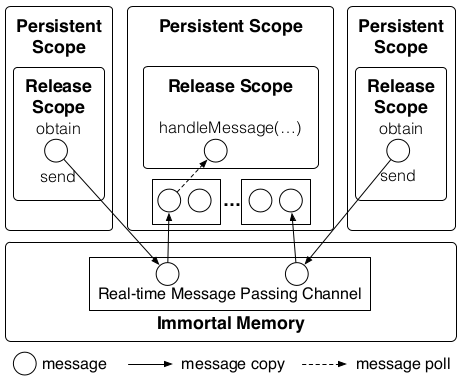
\includegraphics[scale=0.40]{messageChannel}}
	\only<1>{\begin{itemize}
		\item Limitato numero di messaggi in attesa
		\item Trasferibili solo array di tipi primitivi o buffer di byte a dimensione fissa
		\begin{itemize}
			\item In questo modo si mantiene controllata l'occupazione di memoria
		\end{itemize}
		\item I messaggi vengono preallocati sulla base della dimensione della coda 
		\item Se la coda è piena un thread ad alta priorità può ''rubare'' un messaggio
	\end{itemize}}
	\only<2>{\begin{itemize}
		\item I messaggi accodati non sono ancora stati ricevuti, quindi è safe prelevarne uno a bassa priorità
		\begin{itemize}
			\item Il derubato verrà notificato con una eccezione
			\item Il framework assicura che nessun componente abbia un riferimento diretto al messaggio
			\item Chi ha priorità alta non viene bloccato
		\end{itemize}
		\item Il ricevente copia il payload nella sua memoria solo quando accetta il messaggio
		\begin{itemize}
			\item Messaggi accettati uno alla volta
			\item La memoria occupata nel ricevente è tenuta sotto controllo e pulita dopo ogni gestione (release memory)
			\item Una volta ricevuto, il messaggio torna disponibile
		\end{itemize}
		\item Il ricevente non può essere intasato da messaggi in entrata
	\end{itemize}}
\end{frame}
\begin{frame}{RTDroid - Broadcast Channel}
	\only<2>{\centering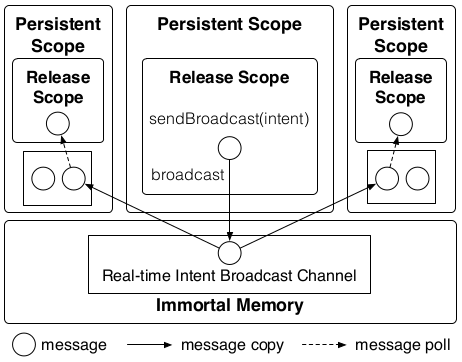
\includegraphics[scale=0.40]{broadcastChannel}}
	\only<1>{\begin{itemize}
		\item Simile ai canali punto a punto, ma in broadcast
		\item Un contatore mantiene il numero di riceventi in attesa
		\begin{itemize}
			\item Conosciuto staticamente grazie a \texttt{manifest.xml}
		\end{itemize}
		\item Messaggio salvato nella memoria immortal e liberato quando tutti lo hanno ricevuto
		\item Utilizzo di memoria limitato e non soggetto a GC
		\begin{itemize}
			\item Nessuna fonte di interferenza
		\end{itemize}
	\end{itemize}}
\end{frame}
\begin{frame}{RTDroid - Cross Context Channel}
	\centering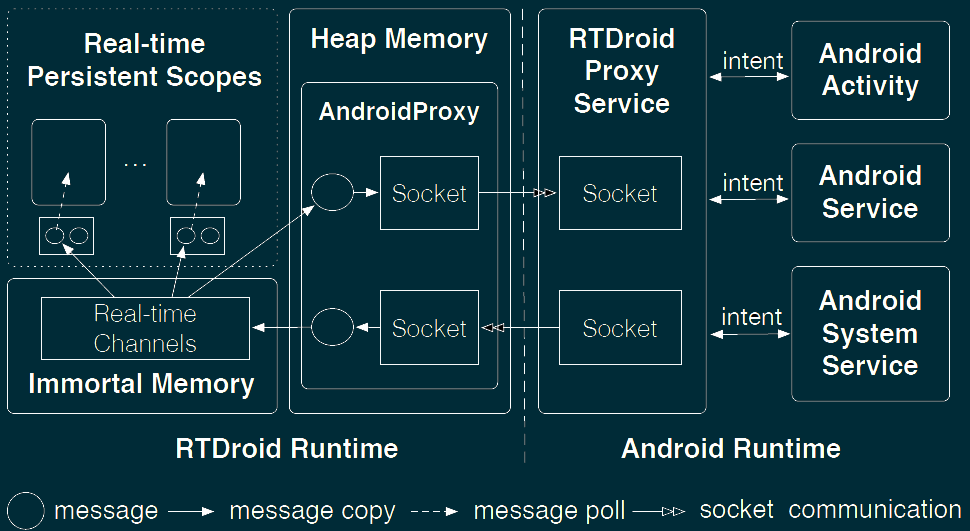
\includegraphics[scale=0.40]{crosscontext}
\end{frame}
\subsection{Valutazione}
\begin{frame}{RTDroid - Prestazioni}
	\only<2>{
		\centering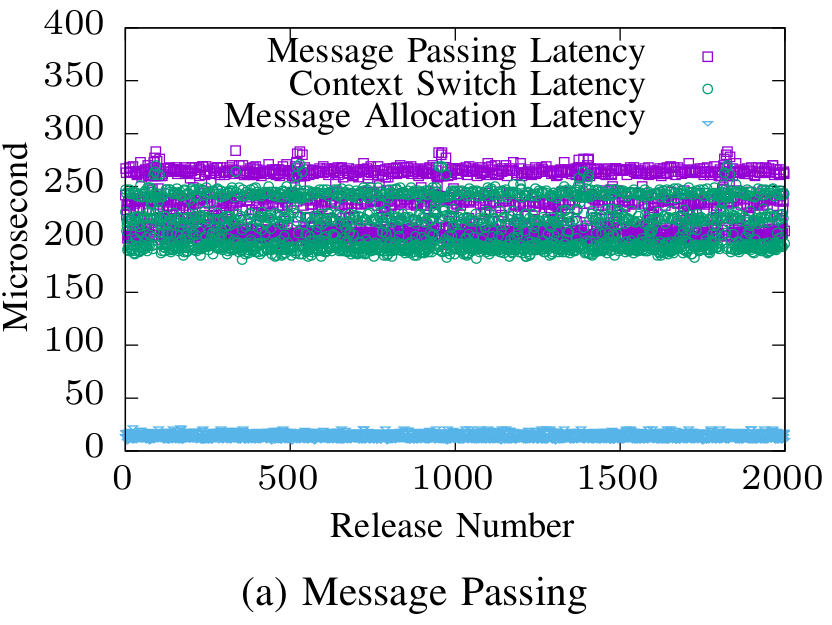
\includegraphics[scale=0.3]{message}
	}

	\only<3>{
		\centering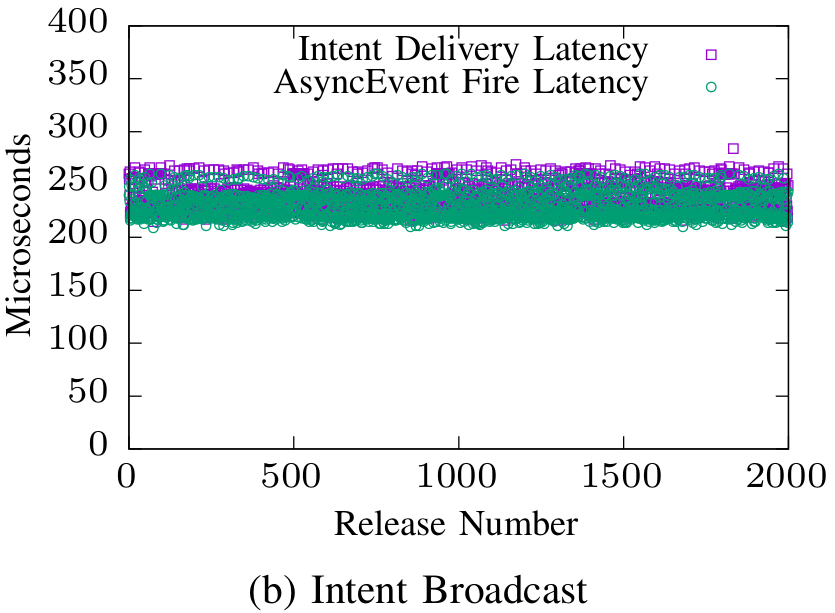
\includegraphics[scale=0.3]{broadcast}
	}
	
	\only<4>{
		\centering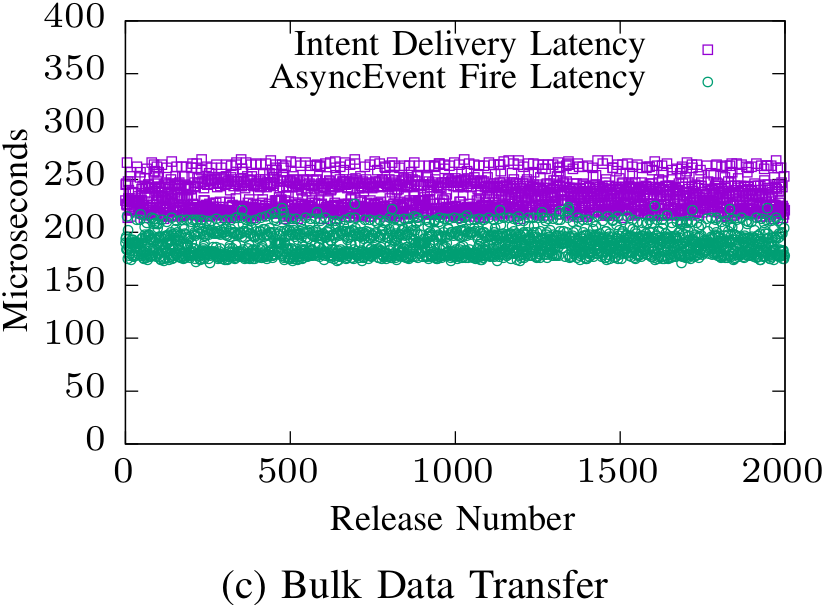
\includegraphics[scale=0.3]{bulk}
	}

	\only<1>{
		\begin{itemize}
			\item Test condotti generando interferenza non real-time
			\begin{itemize}
				\item \textbf{Heap}: allocazione di 512 KB ogni 200 $ms$
				\item \textbf{Calcolo} di $\pi$ ogni 200 $ms$
				\item \textbf{Messaggio} a bassa priorità inviato ogni 200 $ms$
			\end{itemize}
			\item Due thread real-time coinvolti, un sender e un receiver
			\item La latenza rilevata è estremamente limitata
			\begin{itemize}
				\item Le performance sono stabili e prevedibili
			\end{itemize}
		\end{itemize}
	}
\end{frame}
\begin{frame}{RTDroid - Valutazione}
	\only<1>{
		\begin{itemize}
			\item Processing di un segnale audio
			\item $D=28ms$
		\end{itemize}
		\begin{table}[]
			\centering
			\begin{tabular}{c|c|c|}
				\cline{2-3}
				& \multicolumn{2}{c|}{Cochlear Implant} \\ \cline{2-3} 
				& Sampling number   & Deadlines missed   \\ \hline
				\multicolumn{1}{|c|}{Android} & 40.000            & 5160              \\ \hline
				\multicolumn{1}{|c|}{RTSJ}    & 40.000            & 0                 \\ \hline
				\multicolumn{1}{|c|}{RTDroid} & 40.000            & 0                 \\ \hline
			\end{tabular}
		\end{table}
	}

	\only<2>{
		\begin{itemize}
			\item Simulazione controllo aereo
			\begin{itemize}
				\item Task di stabilizzazione
			\end{itemize}
			\item $D=50ms$
		\end{itemize}
		\begin{table}[]
			\centering
			\begin{tabular}{c|c|c|}
				\cline{2-3}
				& \multicolumn{2}{c|}{jPapaBench}   \\ \cline{2-3} 
				& Sampling number & Deadlines missed \\ \hline
				\multicolumn{1}{|c|}{Android} & 92.816          & 14              \\ \hline
				\multicolumn{1}{|c|}{RTSJ}    & 91.791          & 0               \\ \hline
				\multicolumn{1}{|c|}{RTDroid} & 91.840          & 0               \\ \hline
			\end{tabular}
		\end{table}
	}

	\only<3>{
		\begin{itemize}
			\item Rilevazione di rottura tramite analisi di un segnale audio
			\item $D=50ms$
			\item 2MB di dati da analizzare per ogni release
		\end{itemize}
		\begin{table}[]
			\centering
			\begin{tabular}{c|c|c|}
				\cline{2-3}
				& \multicolumn{2}{c|}{Wind Turbine Health Monitor} \\ \cline{2-3} 
				& Sampling numer   & Deadlines missed   \\ \hline
				\multicolumn{1}{|c|}{RTSJ}    & 2295             & 0                 \\ \hline
				\multicolumn{1}{|c|}{RTDroid} & 2295             & 0                 \\ \hline
			\end{tabular}
		\end{table}
	}
\end{frame}
\begin{frame}{RTDroid - Valutazione}
	Vantaggi
	\begin{itemize}
		\item[+] Rispetto delle deadlines
		\item[+] Riduzione della complessità del codice
		\item[+] Supporto real-time per molti componenti
		\item[+] Limiti statici di memoria
	\end{itemize}
	\vspace{10px}
	Svantaggi
	\begin{itemize}
		\item[-] Tantissime modifiche richieste
		\begin{itemize}
			\item Kernel
			\item Libreria C
			\item JVM
		\end{itemize}
		\item[-] Affidamento sui programmatori
	\end{itemize}
\end{frame}

\section{Conclusioni}
\begin{frame}{Conclusioni}
	\begin{itemize}
	\end{itemize}
\end{frame}
\begin{frame}{Conclusioni - Fuchsia}
	\only<1>{
		\vspace{-0.5cm}
		\centering
\includegraphics[scale=0.25]{androidtofuchsia}
	}

	\only<2>{
		\begin{itemize}
			\item Nuovo sistema operativo attualmente in fase di sviluppo
			\item Kernels real-time nativi
			\begin{itemize}
				\item Little kernel per dispositivi con risorse limitate
				\item Magenta (by Google) per dispositivi embedded con vincoli di risorse meno stringenti
				\item Scritti prevalentemente in C/C++
			\end{itemize}
		\end{itemize}
	}
	\only<3>{
		\begin{itemize}
			\item Le applicazioni sono scritte in Dart
			\begin{itemize}
				\item È presente una VM
				\item Tutti gli oggetti sono allocati sullo heap
				\item Due tipi di oggetti
				\begin{itemize}
					\item Short-lived, allocati in un'area chiamata \textit{new generation} la cui collection è ottimizzata e veloce (circa 2 $ms$)
					\item Long-lived, allocati nello heap ``classico''
					\item I primi hanno un tempo di vita molto corto e non occupano molto spazio, quindi sono adatti ad un uso in contesti real-time
				\end{itemize}
				\item Modello di concorrenza a \textit{isolates}, simili agli attori di Scala/Akka
				\begin{itemize}
					\item La comunicazione avviene tramite lo scambio di messaggi e non con memoria condivisa
					\item Facilmente analizzabile staticamente e senza rischio di data races
				\end{itemize}
			\end{itemize}
		\end{itemize}
	}
\end{frame}


\appendix
\makethanks
\renewcommand{\turnOffNumbers}{true} %hide frame numbers in footer
\begin{frame}[noframenumbering]{RTDroid - Funzioni di ripartizione}
	\only<1>{
		\centering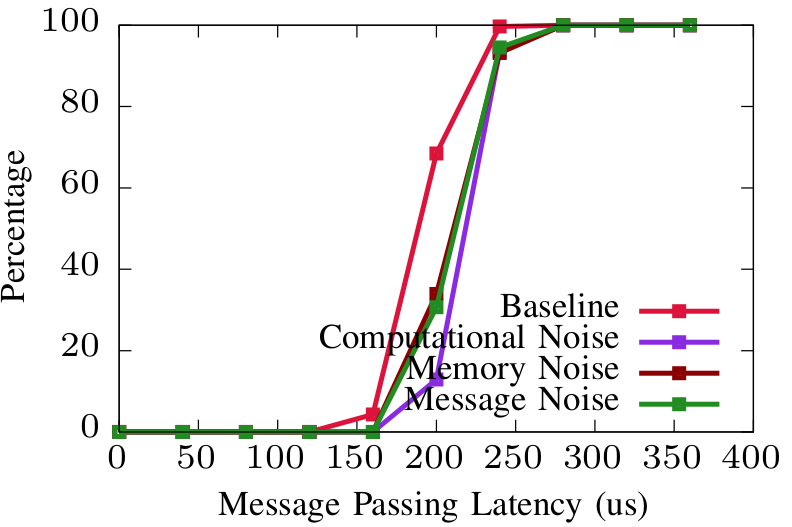
\includegraphics[scale=0.3]{cdfMessage}
	}

	\only<2>{
		\centering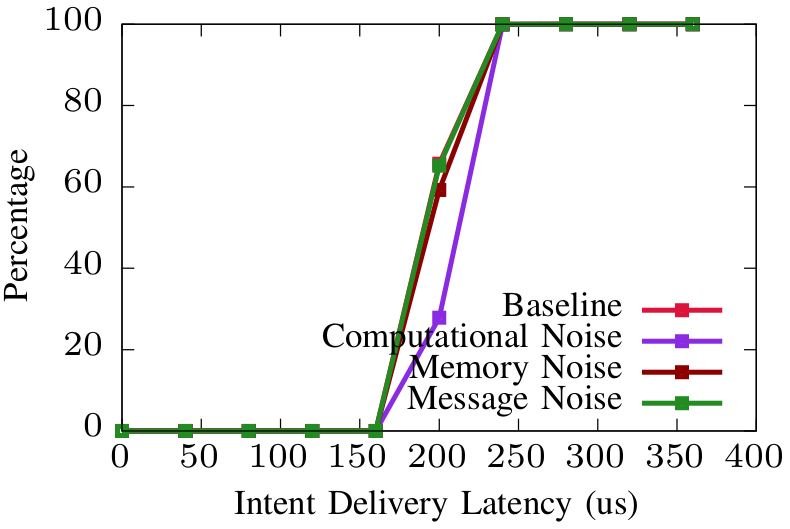
\includegraphics[scale=0.3]{cdfBroadcast}
	}
	
	\only<3>{
		\centering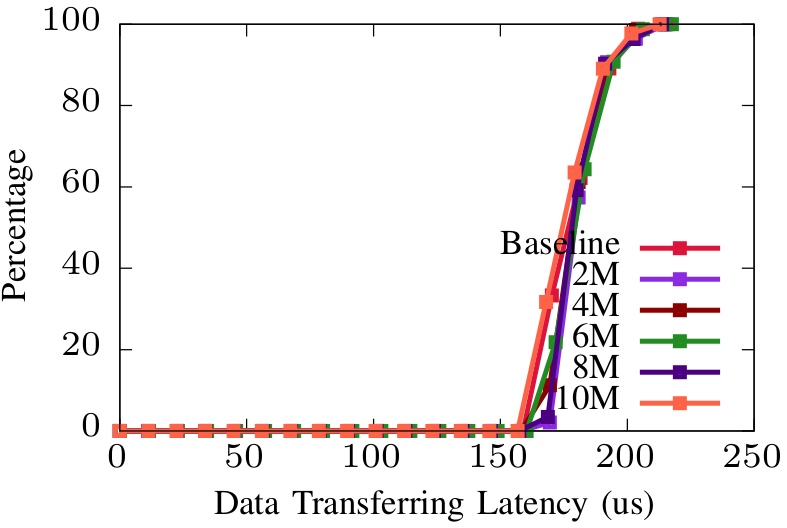
\includegraphics[scale=0.3]{cdfBulk}
	}
\end{frame}
\begin{frame}{RTDroid vs RTSJ}
	\only<1>{
		\centering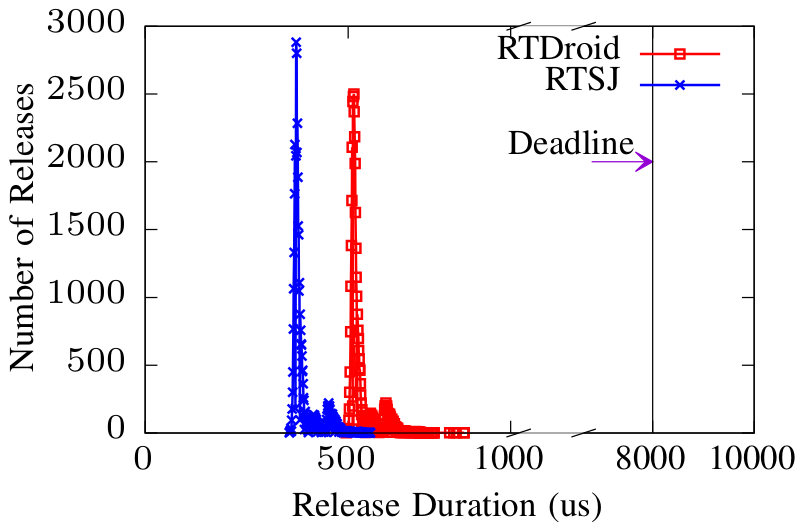
\includegraphics[scale=0.3]{deadlineCochlear}
	}

	\only<2>{
		\centering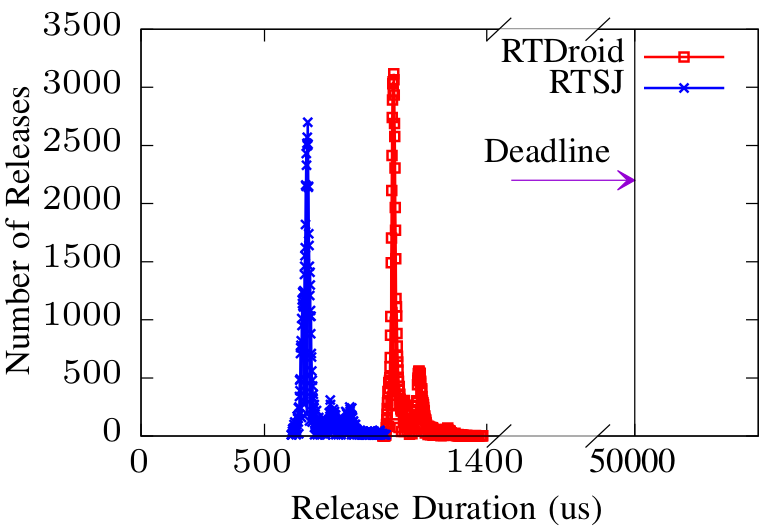
\includegraphics[scale=0.3]{deadlinejPapaBench}
	}
	
	\only<3>{
		\centering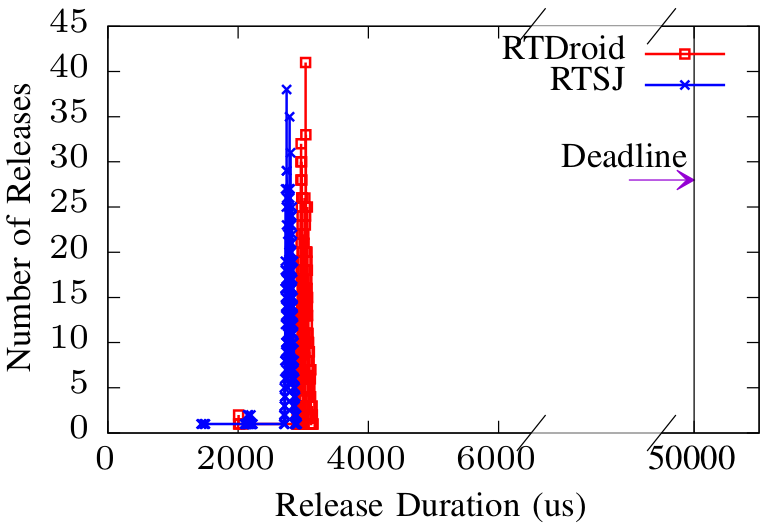
\includegraphics[scale=0.3]{deadlineTurbine}
	}
\end{frame}
\begin{frame}{RTDroid vs Android}
	\only<1>{
		\centering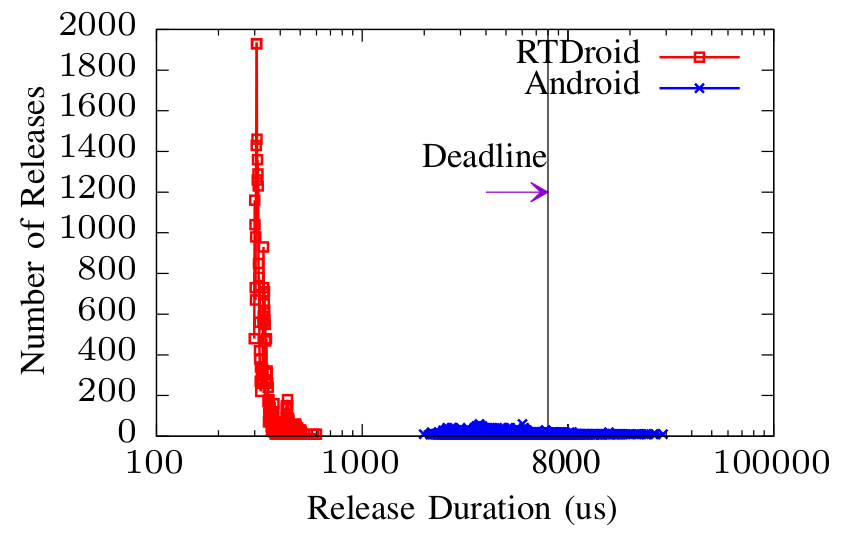
\includegraphics[scale=0.3]{deadlineCochlear2}
	}

	\only<2>{
		\centering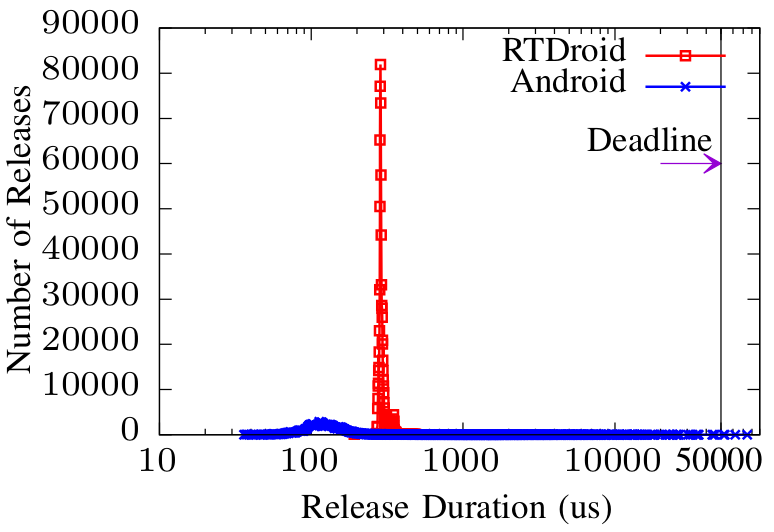
\includegraphics[scale=0.3]{deadlinejPapaBench2}
	}
\end{frame}
\end{document}
